\documentclass[11pt]{beamer}

\usepackage{lmodern}
\usepackage[beamer,customcolors]{hf-tikz}

\tikzset{hl/.style={
    set fill color=red!80!black!40,
    set border color=red!80!black,
  },
}

\addtobeamertemplate{navigation symbols}{}{%
    \usebeamerfont{footline}%
    \usebeamercolor[fg]{footline}%
    \hspace{1em}%
    \insertframenumber/\inserttotalframenumber
}

\usetheme{Montpellier}
\usepackage[utf8]{inputenc}
\usepackage[english,american]{babel}
\usepackage{amsmath}
\usepackage{amsfonts}
\usepackage{amssymb}
\usepackage{graphicx}
\usepackage{booktabs}
\usepackage{float}
\usepackage{multirow}
\usepackage{subcaption}
\usepackage{threeparttable}
\usepackage{pdflscape}
\usepackage{lscape}
\usepackage{array} % for defining a new column type
\usepackage{tabulary}
\newcolumntype{K}[1]{>{\centering\arraybackslash}p{#1}}

	
\author[Francisco Cavalcanti]{Francisco Cavalcanti\\\footnotesize{PUC-Rio}
}

\author{
Flávia  Alfenas\\
\textit{PUC-Rio}\\ \vspace{3mm}
\and  
Francisco Cavalcanti\\
\textit{PUC-Rio}\\ \vspace{3mm}
\and   
Gustavo Gonzaga \\
\textit{PUC-Rio} 
}

\date{Julho, 2020}

\title{Mercado de Trabalho na Amazônia Legal \\ Números Absolutos}

\usepackage{tikz}
\def\checkmark{\tikz\fill[scale=0.4](0,.35) -- (.25,0) -- (1,.7) -- (.25,.15) -- cycle;} 


\newcommand{\quotes}[1]{``#1''}


\setbeamercovered{transparent} 
%\setbeamertemplate{navigation symbols}{} 
%\logo{} 
%\institute{} 
%\date{} 
%\subject{} 
\begin{document}

\newcolumntype{M}{>{\begin{varwidth}{4cm}}l<{\end{varwidth}}} %M is for Maximal column

\begin{frame}
\titlepage
\end{frame}

%\begin{frame}
%\tableofcontents
%\end{frame}

\section{Introdução}

\begin{frame}[label=indice_principal]{Índice Principal}

\begin{itemize}
\item{
	\hyperlink{_estrutura_emprego}{\beamerbutton{Estrutrura do Emprego}} - Descreve a estrutura e evolução do emprego da Amazônia Legal e compara com o resto do Brasil.
	}   
		  
	
\item{
	\hyperlink{_composicao_demografica}{\beamerbutton{Composição Demográfica}} - Esta seção destrincha a estrutura do mercado de trabalho na Amazônia Legal por composições demográficas.
	}  

\end{itemize}

\end{frame}

\section{Estrutura do Emprego}

\begin{frame}[label=_estrutura_emprego]{Estrutura do Emprego}
{\footnotesize Fonte de dados: Dados da PNAD Contínua Trimestral (2012-2020)}
\begin{itemize}
\item{Taxa de ocupação: \hyperlink{_estrutura_emprego_taxa_de_ocupacao}{\beamerbutton{clique aqui}}}
\item{Taxa de informalidade: \hyperlink{_estrutura_emprego_taxa_de_informalidade}{\beamerbutton{clique aqui}}}
\item{Taxa de desemprego: \hyperlink{_estrutura_emprego_taxa_de_desemprego}{\beamerbutton{clique aqui}}}
\item{Taxa de participação: \hyperlink{_estrutura_emprego_taxa_de_participacao}{\beamerbutton{clique aqui}}}
\item{Proporção de militares e estatutários: \hyperlink{_estrutura_emprego_prop_militar}{\beamerbutton{clique aqui}}}
\item{Proporção de empregados sem carteira: \hyperlink{_estrutura_emprego_prop_empregadoSC}{\beamerbutton{clique aqui}}}
\item{Proporção de empregados com carteira: \hyperlink{_estrutura_emprego_prop_empregadoCC}{\beamerbutton{clique aqui}}}
\item{Proporção de empregadores \hyperlink{_estrutura_emprego_prop_empregador}{\beamerbutton{clique aqui}}}
\item{Proporção de conta própria: \hyperlink{_estrutura_emprego_prop_cpropria}{\beamerbutton{clique aqui}}}
\item{Proporção de conta própria que contribui: \hyperlink{_estrutura_emprego_prop_cpropriaC}{\beamerbutton{clique aqui}}}
\item{Proporção de conta própria que não contribui: \hyperlink{_estrutura_emprego_prop_cpropriaNc}{\beamerbutton{clique aqui}}}
\end{itemize}

\begin{small}
\textit{Retornar ao índice principal: \hyperlink{indice_principal}{\beamerbutton{AQUI}} }
\end{small}

\end{frame}

\begin{frame}[label=_estrutura_emprego_taxa_de_ocupacao]{}
\textit{\hyperlink{_estrutura_emprego}{\beamerbutton{Voltar}}}
\begin{figure}
  \centering
  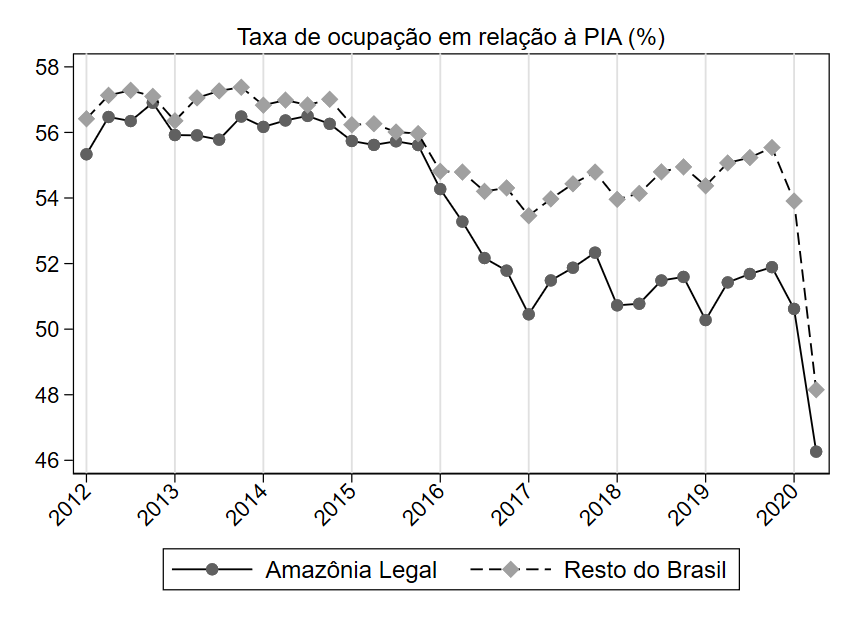
\includegraphics[width=1\linewidth]{../../analysis/output/estrutura_emprego/_estrutura_emprego_taxa_de_ocupacao.png}
  \caption{}
  \label{fig:_estrutura_emprego_taxa_de_ocupacao}
\end{figure}
\end{frame}

\begin{frame}[label=_estrutura_emprego_taxa_de_informalidade]{}
\textit{\hyperlink{_estrutura_emprego}{\beamerbutton{Voltar}}}
\begin{figure}
  \centering
  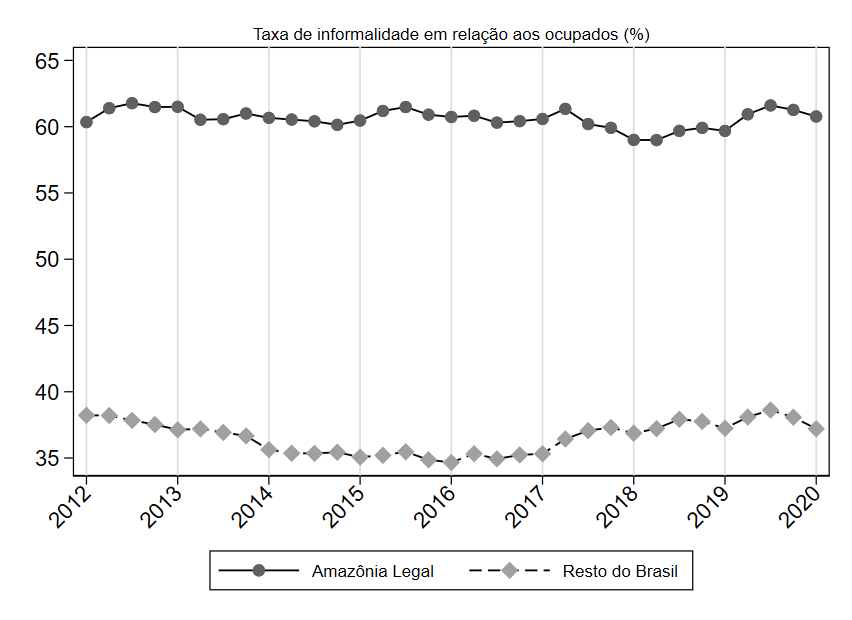
\includegraphics[width=1.0\linewidth]{../../analysis/output/estrutura_emprego/_estrutura_emprego_taxa_de_informalidade.png}
  \caption{}
  \label{fig:_estrutura_emprego_taxa_de_informalidade}
\end{figure}
\end{frame}

\begin{frame}[label=_estrutura_emprego_taxa_de_desemprego]{}
\textit{\hyperlink{_estrutura_emprego}{\beamerbutton{Voltar}}}
\begin{figure}
  \centering
  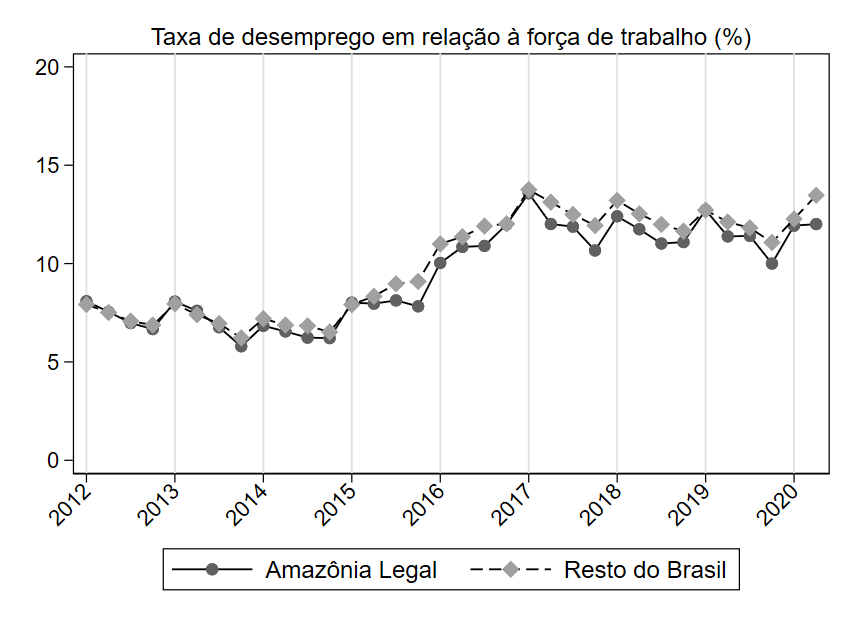
\includegraphics[width=1.0\linewidth]{../../analysis/output/estrutura_emprego/_estrutura_emprego_taxa_de_desemprego.png}
  \caption{}
  \label{fig:_estrutura_emprego_taxa_de_desemprego}
\end{figure}
\end{frame}

\begin{frame}[label=_estrutura_emprego_taxa_de_participacao]{}
\textit{\hyperlink{_estrutura_emprego}{\beamerbutton{Voltar}}}
\begin{figure}
  \centering
  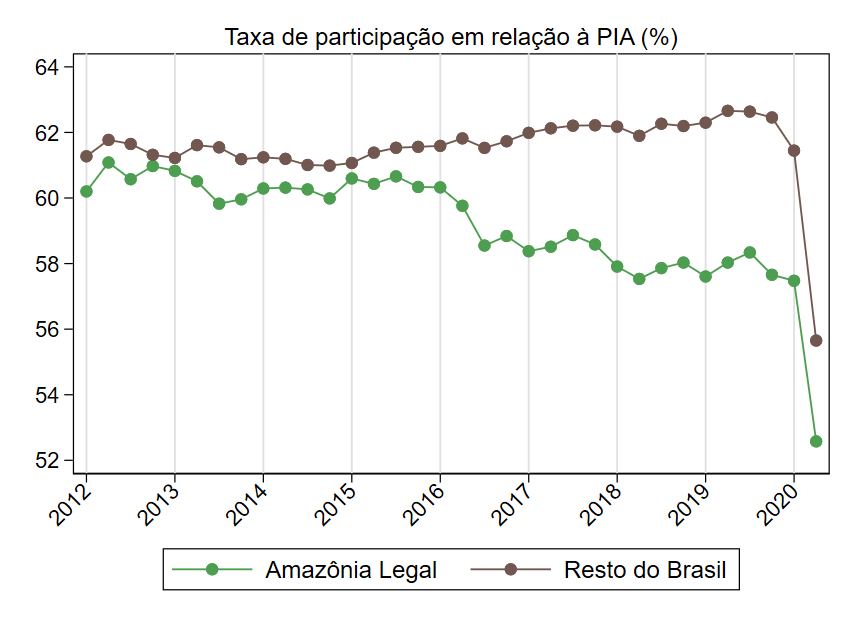
\includegraphics[width=1.0\linewidth]{../../analysis/output/estrutura_emprego/_estrutura_emprego_taxa_de_participacao.png}
  \caption{}
  \label{fig:_estrutura_emprego_taxa_de_participacao}
\end{figure}
\end{frame}


\begin{frame}[label=_estrutura_emprego_prop_militar]{}
\textit{\hyperlink{_estrutura_emprego}{\beamerbutton{Voltar}}}
\begin{figure}
  \centering
  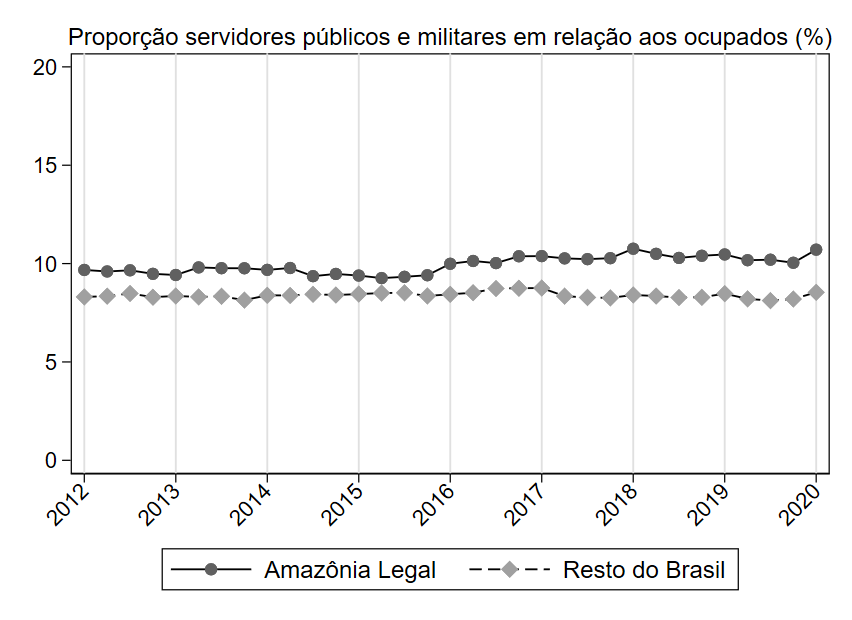
\includegraphics[width=1.0\linewidth]{../../analysis/output/estrutura_emprego/_estrutura_emprego_prop_militar.png}
  \caption{}
  \label{fig:_estrutura_emprego_prop_militar}
\end{figure}
\end{frame}


\begin{frame}[label=_estrutura_emprego_prop_empregadoSC]{}
\textit{\hyperlink{_estrutura_emprego}{\beamerbutton{Voltar}}}
\begin{figure}
  \centering
  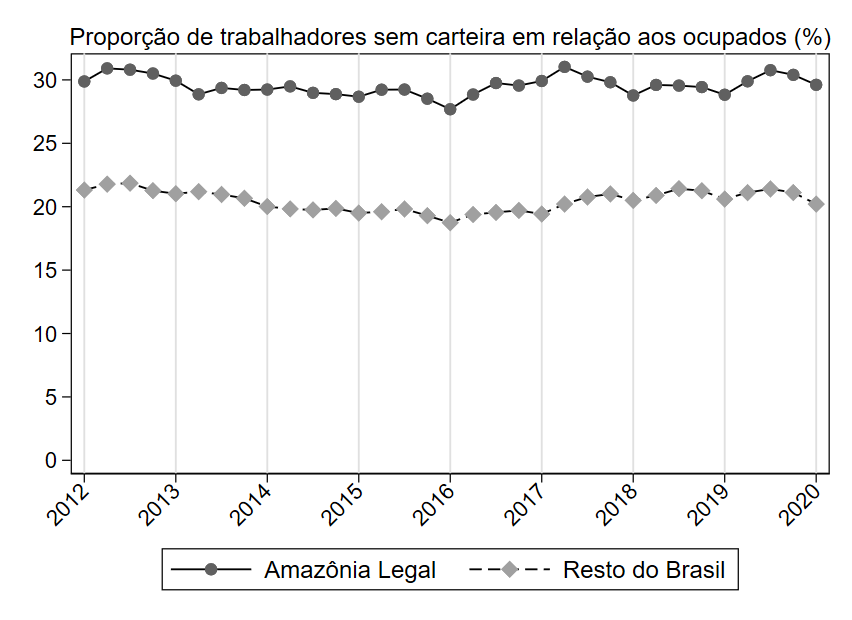
\includegraphics[width=1.0\linewidth]{../../analysis/output/estrutura_emprego/_estrutura_emprego_prop_empregadoSC.png}
  \caption{}
  \label{fig:_estrutura_emprego_prop_empregadoSC}
\end{figure}
\end{frame}

\begin{frame}[label=_estrutura_emprego_prop_empregadoCC]{}
\textit{\hyperlink{_estrutura_emprego}{\beamerbutton{Voltar}}}
\begin{figure}
  \centering
  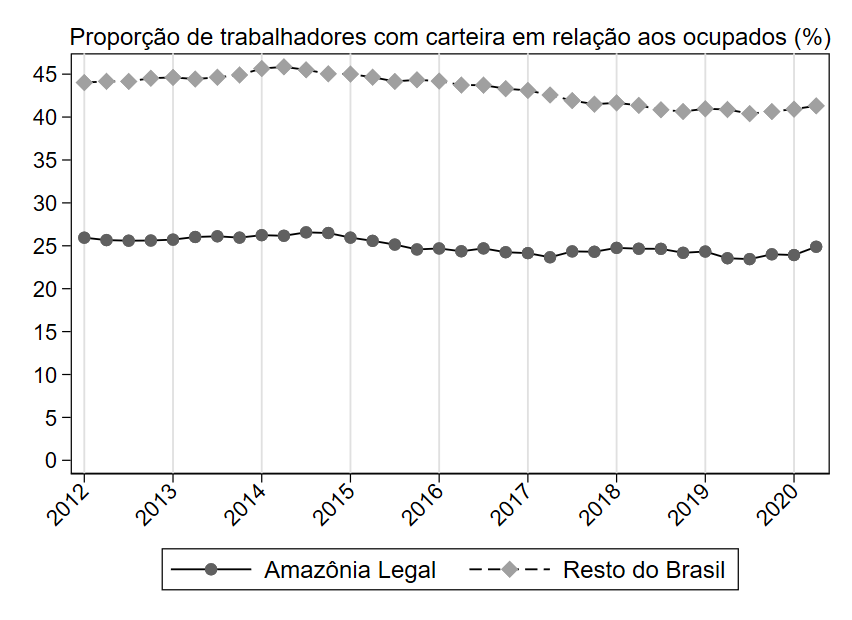
\includegraphics[width=1.0\linewidth]{../../analysis/output/estrutura_emprego/_estrutura_emprego_prop_empregadoCC.png}
  \caption{}
  \label{fig:_estrutura_emprego_prop_empregadoCC}
\end{figure}
\end{frame}

\begin{frame}[label=_estrutura_emprego_prop_empregador]{}
\textit{\hyperlink{_estrutura_emprego}{\beamerbutton{Voltar}}}
\begin{figure}
  \centering
  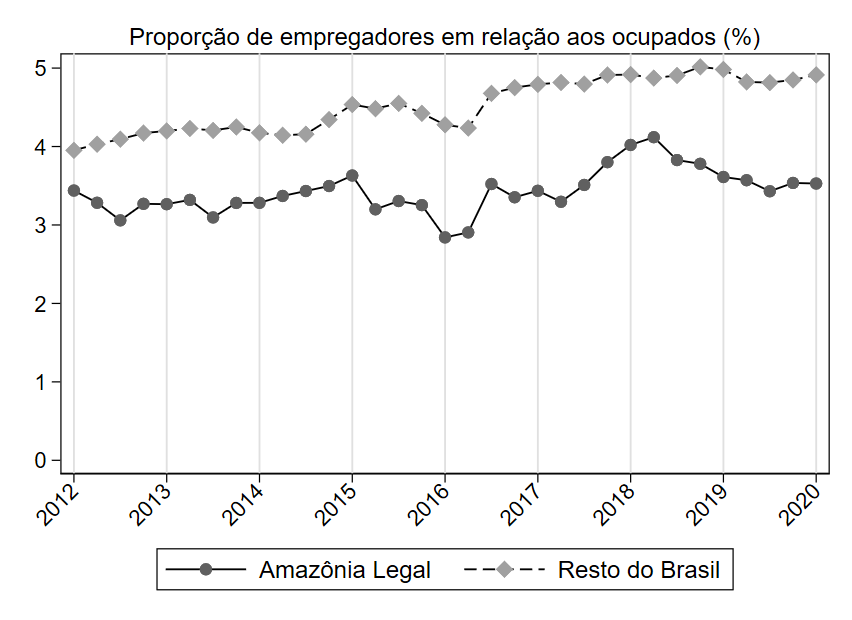
\includegraphics[width=1.0\linewidth]{../../analysis/output/estrutura_emprego/_estrutura_emprego_prop_empregador.png}
  \caption{}
  \label{fig:_estrutura_emprego_prop_empregador}
\end{figure}
\end{frame}



\begin{frame}[label=_estrutura_emprego_prop_cpropria]{}
\textit{\hyperlink{_estrutura_emprego}{\beamerbutton{Voltar}}}
\begin{figure}
  \centering
  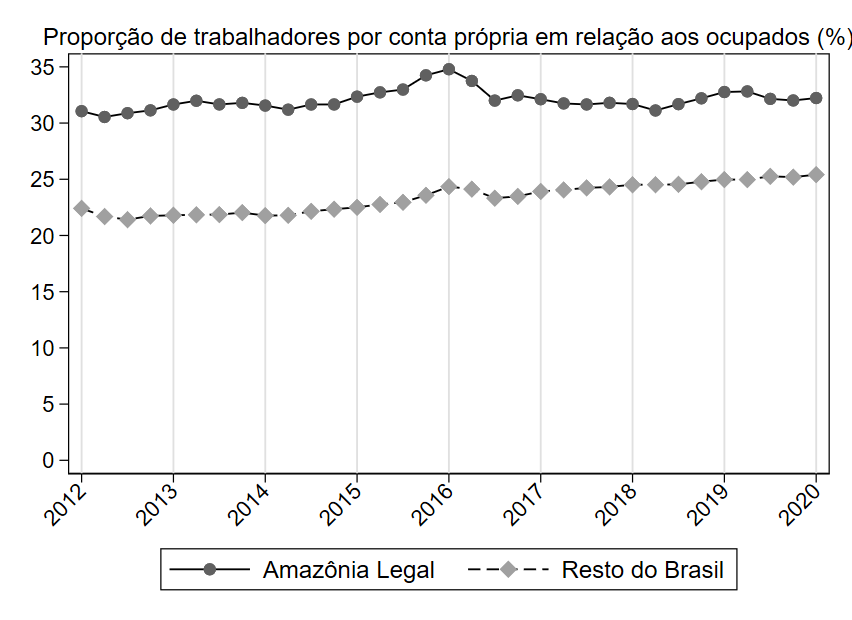
\includegraphics[width=1.0\linewidth]{../../analysis/output/estrutura_emprego/_estrutura_emprego_prop_cpropria.png}
  \caption{}
  \label{fig:_estrutura_emprego_prop_cpropria}
\end{figure}
\end{frame}

\begin{frame}[label=_estrutura_emprego_prop_cpropriaC]{}
\textit{\hyperlink{_estrutura_emprego}{\beamerbutton{Voltar}}}
\begin{figure}
  \centering
  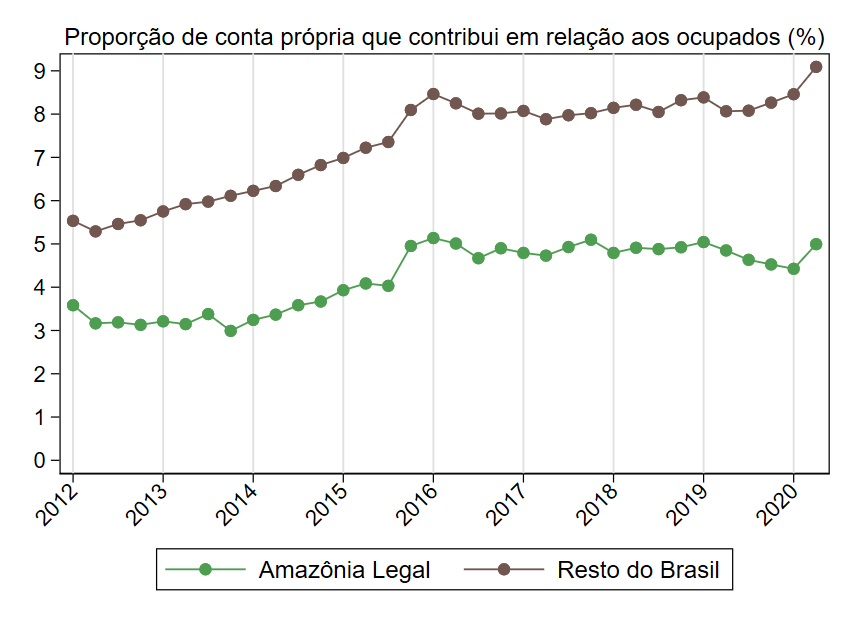
\includegraphics[width=1.0\linewidth]{../../analysis/output/estrutura_emprego/_estrutura_emprego_prop_cpropriaC.png}
  \caption{}
  \label{fig:_estrutura_emprego_prop_cpropriaC}
\end{figure}
\end{frame}

\begin{frame}[label=_estrutura_emprego_prop_cpropriaNc]{}
\textit{\hyperlink{_estrutura_emprego}{\beamerbutton{Voltar}}}
\begin{figure}
  \centering
  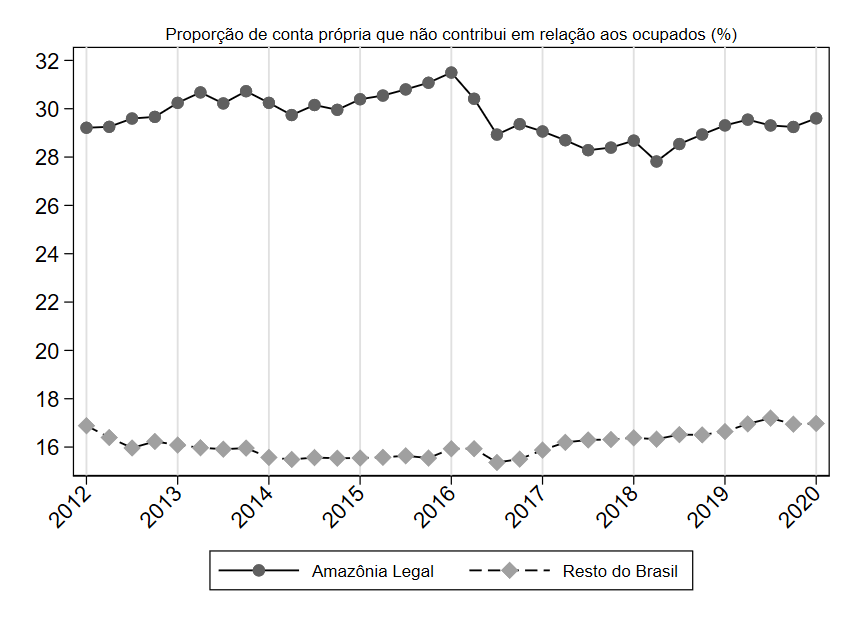
\includegraphics[width=1.0\linewidth]{../../analysis/output/estrutura_emprego/_estrutura_emprego_prop_cpropriaNc.png}
  \caption{}
  \label{fig:_estrutura_emprego_prop_cpropriaNc}
\end{figure}
\end{frame}


\section{Composição Demográfica}

\begin{frame}[label=_composicao_demografica]{Composição Demográfica}
{\footnotesize Fonte de dados: Dados da PNAD Contínua Anual (2012-2019)}



\begin{itemize}
\item{
	\hyperlink{_composicao_demografica_raca}{\beamerbutton{Raça}}
	}   
		
\item{
	\hyperlink{_composicao_demografica_genero}{\beamerbutton{Gênero}}
	}  
	
\item{
	\hyperlink{_composicao_demografica_faixa_etaria}{\beamerbutton{Faixa etária}}
	}  
	
\item{
	\hyperlink{_composicao_demografica_educacao}{\beamerbutton{Educação}} 
	}  
	
\item{
	\hyperlink{_composicao_demografica_setor}{\beamerbutton{Setor ocupacional}}
	}  
	
\item{
	\hyperlink{_composicao_demografica_regiao_metro}{\beamerbutton{Regiões metropolitanas}} 
	}
\item{
	\hyperlink{_composicao_demografica_rural_urbano}{\beamerbutton{Zona rural vs. zona urbana}} 
	} 	  

\end{itemize}
\begin{small}
\textit{Retornar ao índice principal: \hyperlink{indice_principal}{\beamerbutton{AQUI}} }
\end{small}
\end{frame}


\begin{frame}[label=_composicao_demografica_raca]{Composição Demográfica: Raça}
{\footnotesize Fonte de dados: Dados da PNAD Contínua Trimestral (2012-2020)}
\begin{itemize}
\item{Taxa de ocupação: \hyperlink{_composicao_demografica_raca_taxa_de_ocupacao}{\beamerbutton{clique aqui}}}
\item{Taxa de informalidade: \hyperlink{_composicao_demografica_raca_taxa_de_informalidade}{\beamerbutton{clique aqui}}}
\item{Taxa de desemprego: \hyperlink{_composicao_demografica_raca_taxa_de_desemprego}{\beamerbutton{clique aqui}}}
\item{Taxa de participação: \hyperlink{_composicao_demografica_raca_taxa_de_participacao}{\beamerbutton{clique aqui}}}
\item{Proporção de servidores públicos e militares: \hyperlink{_composicao_demografica_raca_prop_militar}{\beamerbutton{clique aqui}}}
\item{Proporção de empregados sem carteira: \hyperlink{_composicao_demografica_raca_prop_empregadoSC}{\beamerbutton{clique aqui}}}
\item{Proporção de empregados com carteira: \hyperlink{_composicao_demografica_raca_prop_empregadoCC}{\beamerbutton{clique aqui}}}
\item{Proporção de empregadores \hyperlink{_composicao_demografica_raca_prop_empregador}{\beamerbutton{clique aqui}}}
\item{Proporção de conta própria: \hyperlink{_composicao_demografica_raca_prop_cpropria}{\beamerbutton{clique aqui}}}
\item{Proporção de conta própria que contribui: \hyperlink{_composicao_demografica_raca_prop_cpropriaC}{\beamerbutton{clique aqui}}}
\item{Proporção de conta própria que não contribui: \hyperlink{_composicao_demografica_raca_prop_cpropriaNc}{\beamerbutton{clique aqui}}}
\end{itemize}

\begin{small}
\textit{Retornar ao índice principal da composição demográfica: \hyperlink{_composicao_demografica}{\beamerbutton{AQUI}} }
\end{small}

\end{frame}

\begin{frame}[label=_composicao_demografica_raca_taxa_de_ocupacao]{}
\textit{\hyperlink{_composicao_demografica_raca}{\beamerbutton{Voltar}}}
\begin{figure}
  \centering
  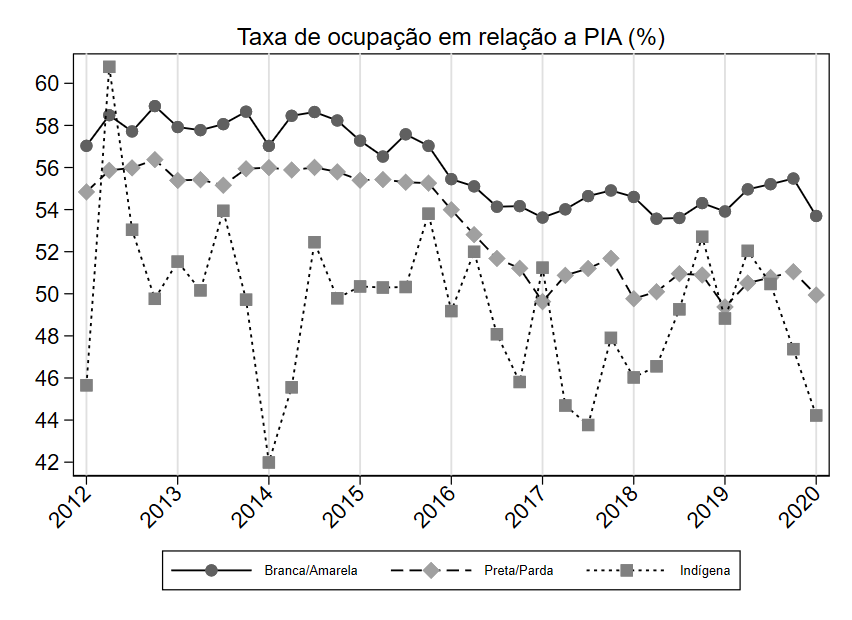
\includegraphics[width=1\linewidth]{../../analysis/output/composicao_demografica/raca/_composicao_demografica_raca_taxa_de_ocupacao.png}
  \caption{}
  \label{fig:_composicao_demografica_raca_taxa_de_ocupacao}
\end{figure}
\end{frame}

\begin{frame}[label=_composicao_demografica_raca_taxa_de_informalidade]{}
\textit{\hyperlink{_composicao_demografica_raca}{\beamerbutton{Voltar}}}
\begin{figure}
  \centering
  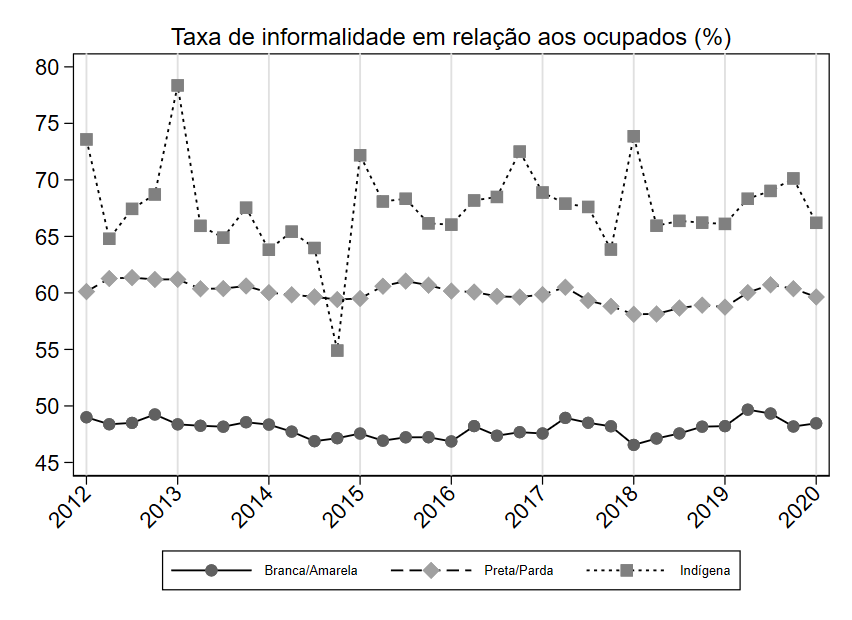
\includegraphics[width=1.0\linewidth]{../../analysis/output/composicao_demografica/raca/_composicao_demografica_raca_taxa_de_informalidade.png}
  \caption{}
  \label{fig:_composicao_demografica_raca_taxa_de_informalidade}
\end{figure}
\end{frame}

\begin{frame}[label=_composicao_demografica_raca_taxa_de_desemprego]{}
\textit{\hyperlink{_composicao_demografica_raca}{\beamerbutton{Voltar}}}
\begin{figure}
  \centering
  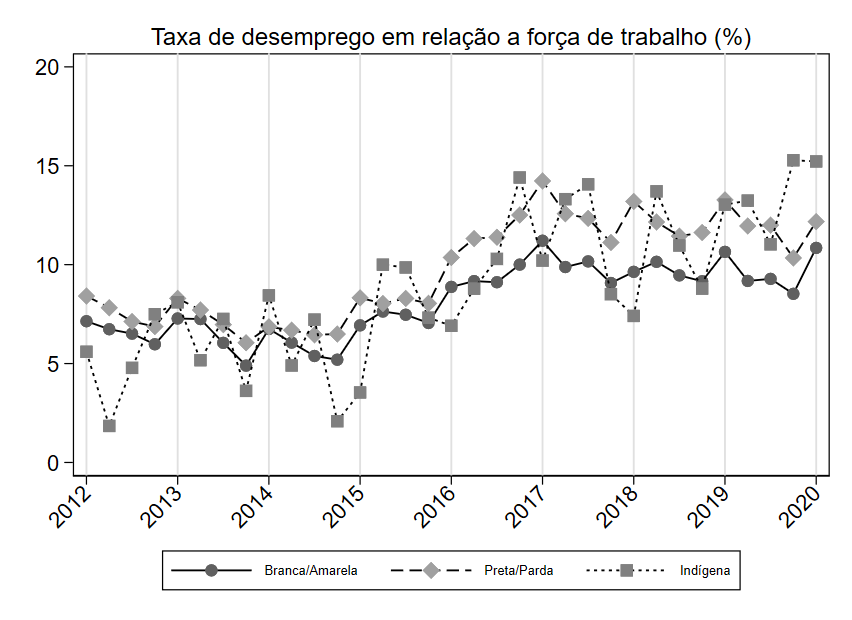
\includegraphics[width=1.0\linewidth]{../../analysis/output/composicao_demografica/raca/_composicao_demografica_raca_taxa_de_desemprego.png}
  \caption{}
  \label{fig:_composicao_demografica_raca_taxa_de_desemprego}
\end{figure}
\end{frame}

\begin{frame}[label=_composicao_demografica_raca_taxa_de_participacao]{}
\textit{\hyperlink{_composicao_demografica_raca}{\beamerbutton{Voltar}}}
\begin{figure}
  \centering
  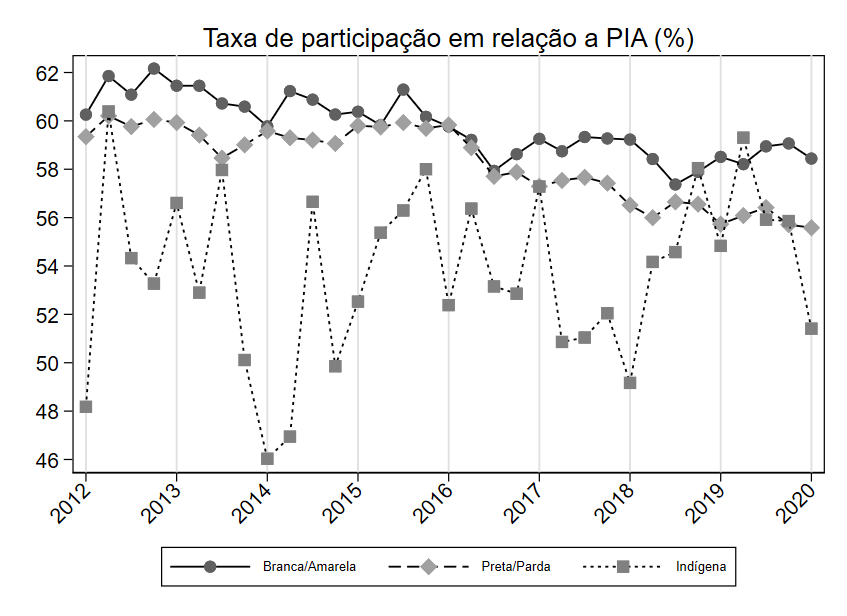
\includegraphics[width=1.0\linewidth]{../../analysis/output/composicao_demografica/raca/_composicao_demografica_raca_taxa_de_participacao.png}
  \caption{}
  \label{fig:_composicao_demografica_raca_taxa_de_participacao}
\end{figure}
\end{frame}

\begin{frame}[label=_composicao_demografica_raca_prop_militar]{}
\textit{\hyperlink{_composicao_demografica_raca}{\beamerbutton{Voltar}}}
\begin{figure}
  \centering
  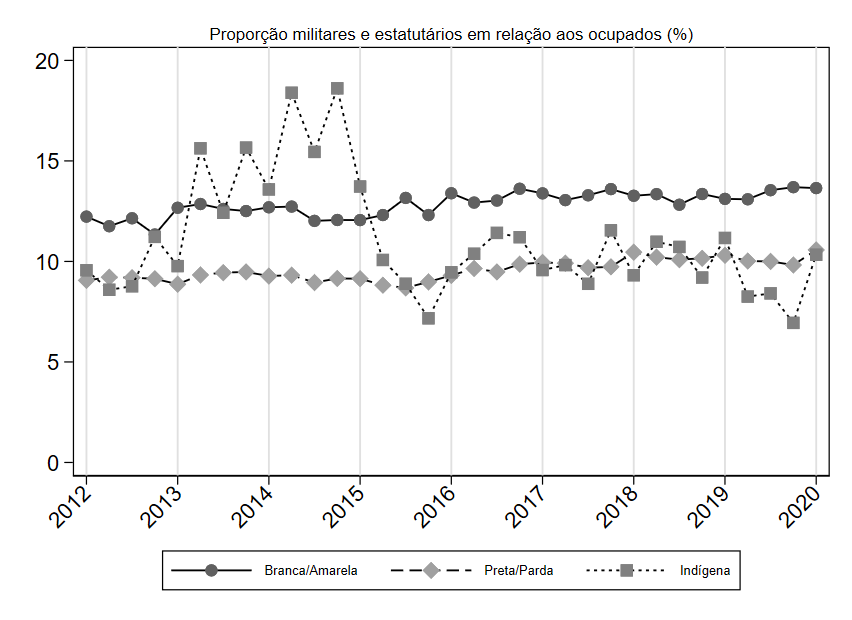
\includegraphics[width=1.0\linewidth]{../../analysis/output/composicao_demografica/raca/_composicao_demografica_raca_prop_militar.png}
  \caption{}
  \label{fig:_composicao_demografica_raca_prop_militar}
\end{figure}
\end{frame}


\begin{frame}[label=_composicao_demografica_raca_prop_empregadoSC]{}
\textit{\hyperlink{_composicao_demografica_raca}{\beamerbutton{Voltar}}}
\begin{figure}
  \centering
  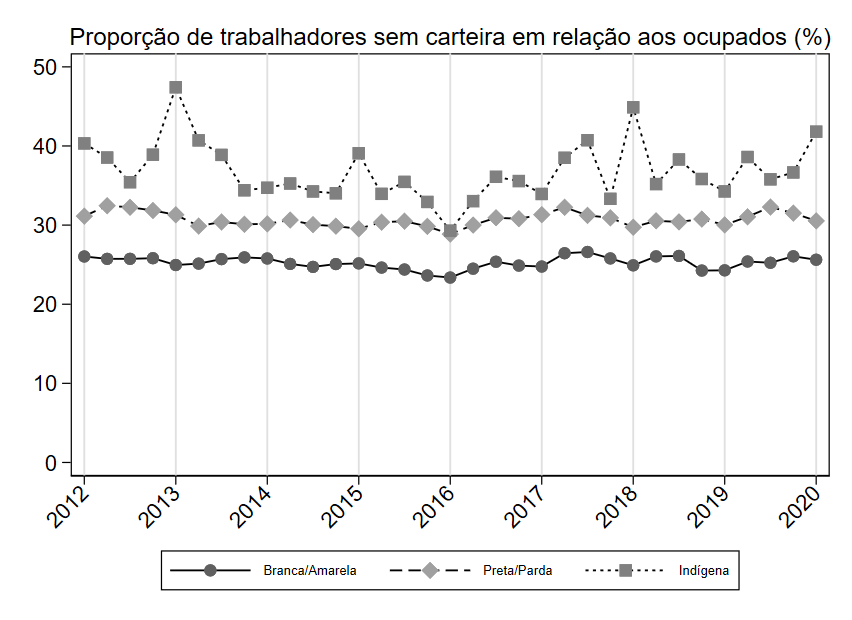
\includegraphics[width=1.0\linewidth]{../../analysis/output/composicao_demografica/raca/_composicao_demografica_raca_prop_empregadoSC.png}
  \caption{}
  \label{fig:_composicao_demografica_raca_prop_empregadoSC}
\end{figure}
\end{frame}

\begin{frame}[label=_composicao_demografica_raca_prop_empregadoCC]{}
\textit{\hyperlink{_composicao_demografica_raca}{\beamerbutton{Voltar}}}
\begin{figure}
  \centering
  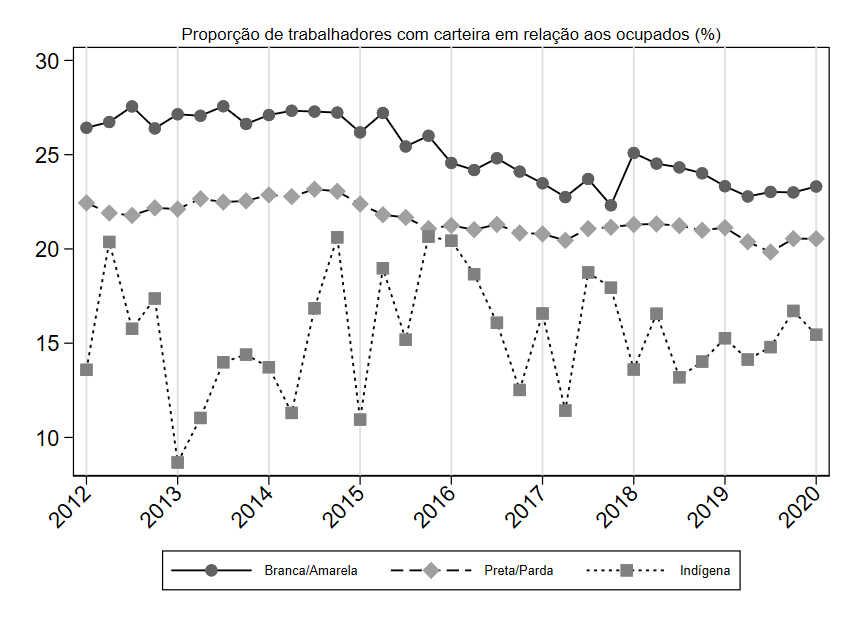
\includegraphics[width=1.0\linewidth]{../../analysis/output/composicao_demografica/raca/_composicao_demografica_raca_prop_empregadoCC.png}
  \caption{}
  \label{fig:_composicao_demografica_raca_prop_empregadoCC}
\end{figure}
\end{frame}

\begin{frame}[label=_composicao_demografica_raca_prop_empregador]{}
\textit{\hyperlink{_composicao_demografica_raca}{\beamerbutton{Voltar}}}
\begin{figure}
  \centering
  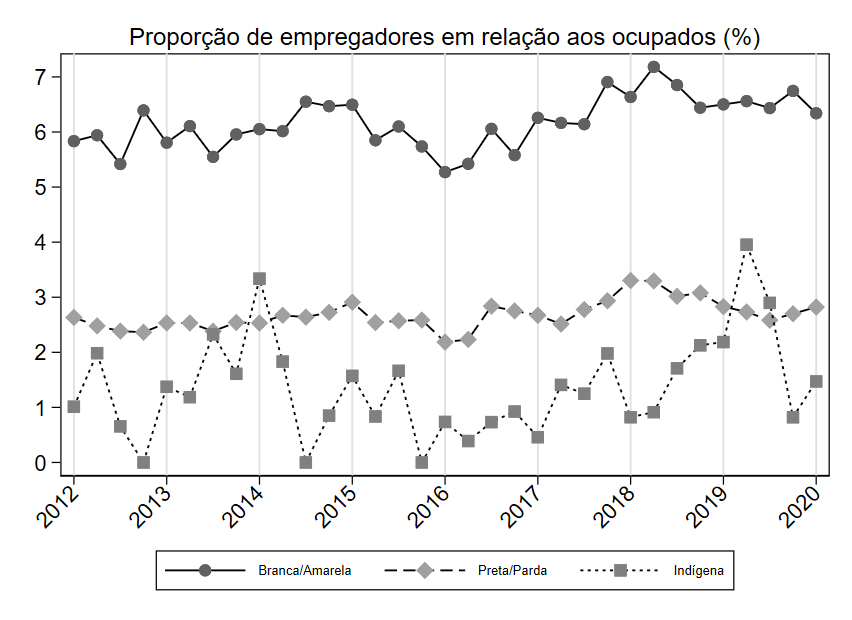
\includegraphics[width=1.0\linewidth]{../../analysis/output/composicao_demografica/raca/_composicao_demografica_raca_prop_empregador.png}
  \caption{}
  \label{fig:_composicao_demografica_raca_prop_empregador}
\end{figure}
\end{frame}



\begin{frame}[label=_composicao_demografica_raca_prop_cpropria]{}
\textit{\hyperlink{_composicao_demografica_raca}{\beamerbutton{Voltar}}}
\begin{figure}
  \centering
  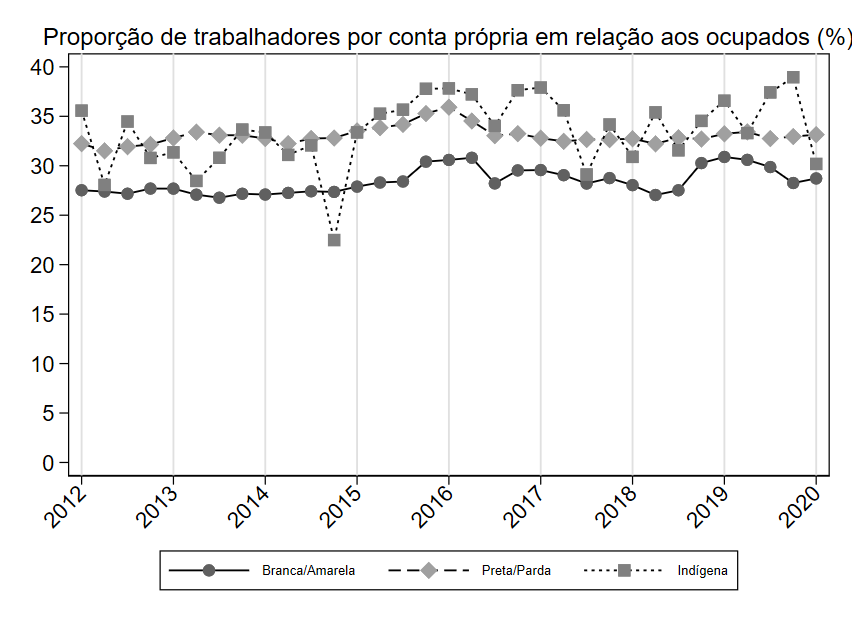
\includegraphics[width=1.0\linewidth]{../../analysis/output/composicao_demografica/raca/_composicao_demografica_raca_prop_cpropria.png}
  \caption{}
  \label{fig:_composicao_demografica_raca_prop_cpropria}
\end{figure}
\end{frame}

\begin{frame}[label=_composicao_demografica_raca_prop_cpropriaC]{}
\textit{\hyperlink{_composicao_demografica_raca}{\beamerbutton{Voltar}}}
\begin{figure}
  \centering
  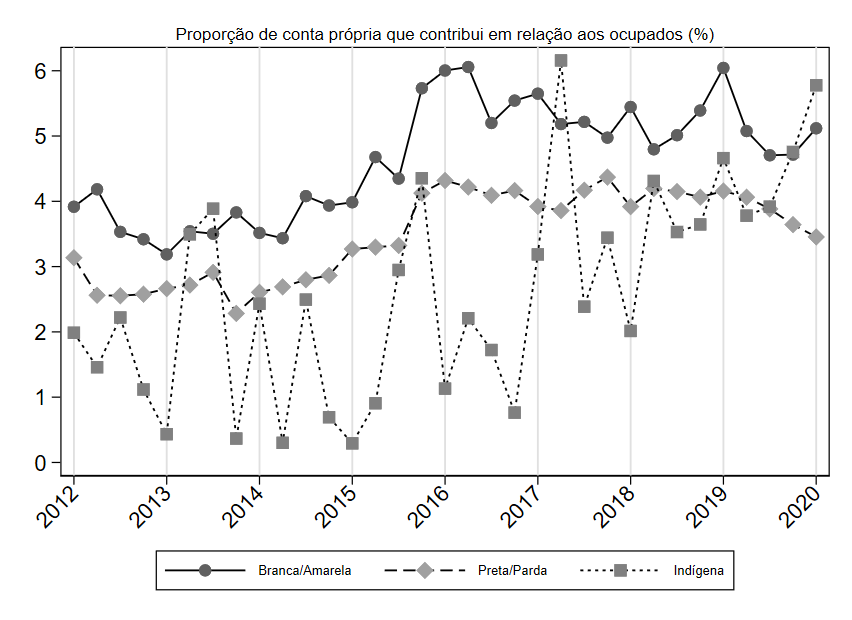
\includegraphics[width=1.0\linewidth]{../../analysis/output/composicao_demografica/raca/_composicao_demografica_raca_prop_cpropriaC.png}
  \caption{}
  \label{fig:_composicao_demografica_raca_prop_cpropriaC}
\end{figure}
\end{frame}

\begin{frame}[label=_composicao_demografica_raca_prop_cpropriaNc]{}
\textit{\hyperlink{_composicao_demografica_raca}{\beamerbutton{Voltar}}}
\begin{figure}
  \centering
  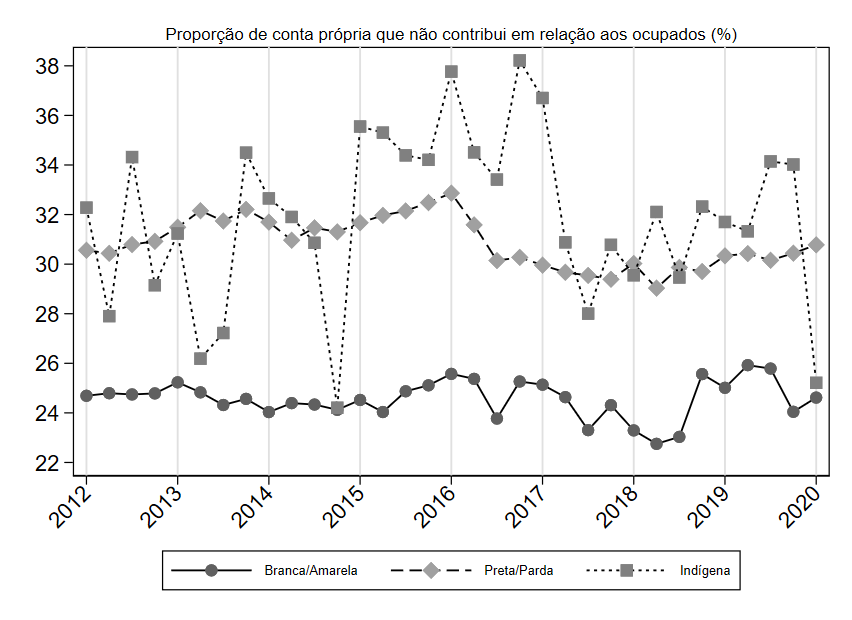
\includegraphics[width=1.0\linewidth]{../../analysis/output/composicao_demografica/raca/_composicao_demografica_raca_prop_cpropriaNc.png}
  \caption{}
  \label{fig:_composicao_demografica_raca_prop_cpropriaNc}
\end{figure}
\end{frame}
\begin{frame}[label=_composicao_demografica_genero]{Composição Demográfica: Gênero}
{\footnotesize Fonte de dados: Dados da PNAD Contínua Trimestral (2012-2020)}
\begin{itemize}
\item{Taxa de ocupação: \hyperlink{_composicao_demografica_genero_taxa_de_ocupacao}{\beamerbutton{clique aqui}}}
\item{Taxa de informalidade: \hyperlink{_composicao_demografica_genero_taxa_de_informalidade}{\beamerbutton{clique aqui}}}
\item{Taxa de desemprego: \hyperlink{_composicao_demografica_genero_taxa_de_desemprego}{\beamerbutton{clique aqui}}}
\item{Taxa de participação: \hyperlink{_composicao_demografica_genero_taxa_de_participacao}{\beamerbutton{clique aqui}}}
\item{Proporção de militares e estatutários: \hyperlink{_composicao_demografica_genero_prop_militar}{\beamerbutton{clique aqui}}}
\item{Proporção de empregados sem carteira: \hyperlink{_composicao_demografica_genero_prop_empregadoSC}{\beamerbutton{clique aqui}}}
\item{Proporção de empregados com carteira: \hyperlink{_composicao_demografica_genero_prop_empregadoCC}{\beamerbutton{clique aqui}}}
\item{Proporção de empregadores \hyperlink{_composicao_demografica_genero_prop_empregador}{\beamerbutton{clique aqui}}}
\item{Proporção de conta própria: \hyperlink{_composicao_demografica_genero_prop_cpropria}{\beamerbutton{clique aqui}}}
\item{Proporção de conta própria que contribui: \hyperlink{_composicao_demografica_genero_prop_cpropriaC}{\beamerbutton{clique aqui}}}
\item{Proporção de conta própria que não contribui: \hyperlink{_composicao_demografica_genero_prop_cpropriaNc}{\beamerbutton{clique aqui}}}
\end{itemize}

\begin{small}
\textit{Retornar ao índice principal da composição demográfica: \hyperlink{_composicao_demografica}{\beamerbutton{AQUI}} }
\end{small}

\end{frame}

\begin{frame}[label=_composicao_demografica_genero_taxa_de_ocupacao]{}
\textit{\hyperlink{_composicao_demografica_genero}{\beamerbutton{Voltar}}}
\begin{figure}
  \centering
  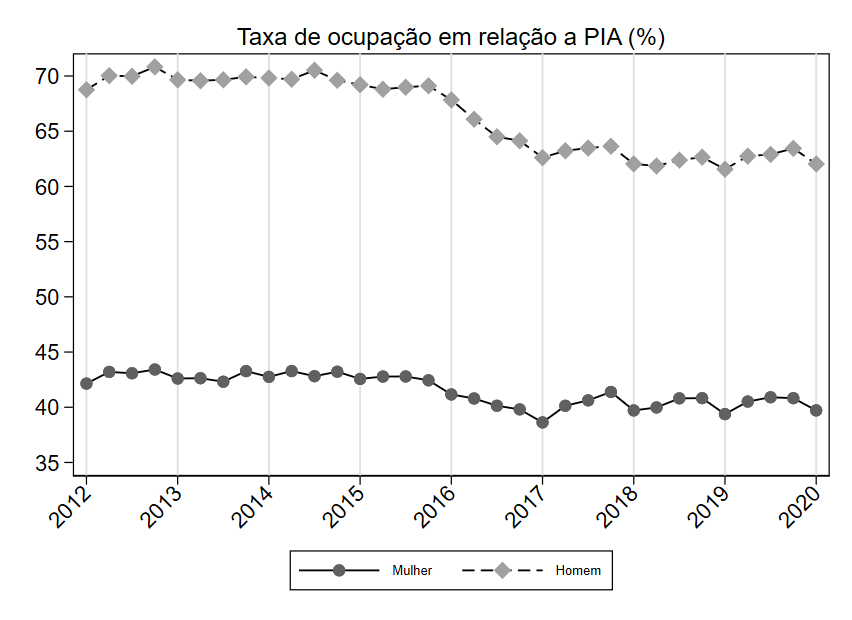
\includegraphics[width=1\linewidth]{../../analysis/output/composicao_demografica/genero/_composicao_demografica_genero_taxa_de_ocupacao.png}
  \caption{}
  \label{fig:_composicao_demografica_genero_taxa_de_ocupacao}
\end{figure}
\end{frame}

\begin{frame}[label=_composicao_demografica_genero_taxa_de_informalidade]{}
\textit{\hyperlink{_composicao_demografica_genero}{\beamerbutton{Voltar}}}
\begin{figure}
  \centering
  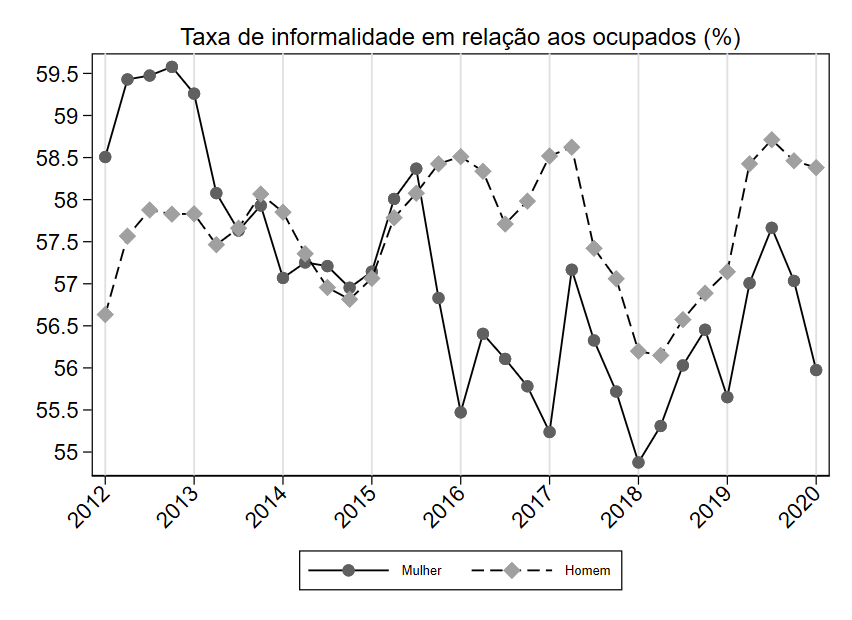
\includegraphics[width=1.0\linewidth]{../../analysis/output/composicao_demografica/genero/_composicao_demografica_genero_taxa_de_informalidade.png}
  \caption{}
  \label{fig:_composicao_demografica_genero_taxa_de_informalidade}
\end{figure}
\end{frame}

\begin{frame}[label=_composicao_demografica_genero_taxa_de_desemprego]{}
\textit{\hyperlink{_composicao_demografica_genero}{\beamerbutton{Voltar}}}
\begin{figure}
  \centering
  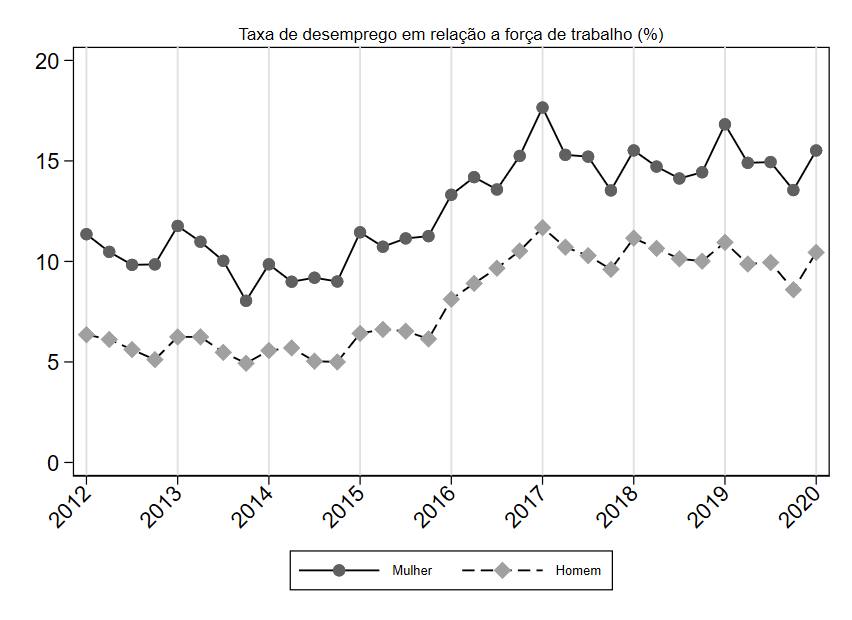
\includegraphics[width=1.0\linewidth]{../../analysis/output/composicao_demografica/genero/_composicao_demografica_genero_taxa_de_desemprego.png}
  \caption{}
  \label{fig:_composicao_demografica_genero_taxa_de_desemprego}
\end{figure}
\end{frame}

\begin{frame}[label=_composicao_demografica_genero_taxa_de_participacao]{}
\textit{\hyperlink{_composicao_demografica_genero}{\beamerbutton{Voltar}}}
\begin{figure}
  \centering
  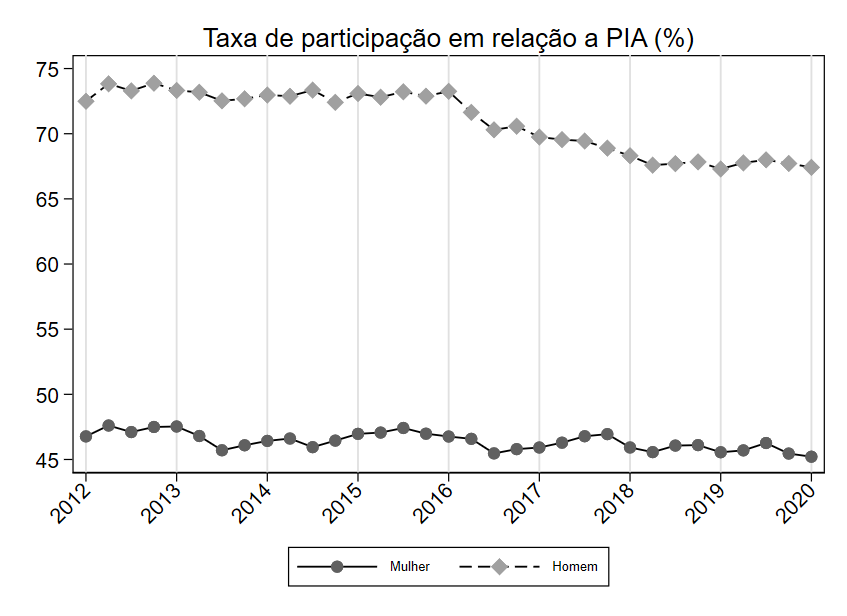
\includegraphics[width=1.0\linewidth]{../../analysis/output/composicao_demografica/genero/_composicao_demografica_genero_taxa_de_participacao.png}
  \caption{}
  \label{fig:_composicao_demografica_genero_taxa_de_participacao}
\end{figure}
\end{frame}

\begin{frame}[label=_composicao_demografica_genero_prop_militar]{}
\textit{\hyperlink{_composicao_demografica_genero}{\beamerbutton{Voltar}}}
\begin{figure}
  \centering
  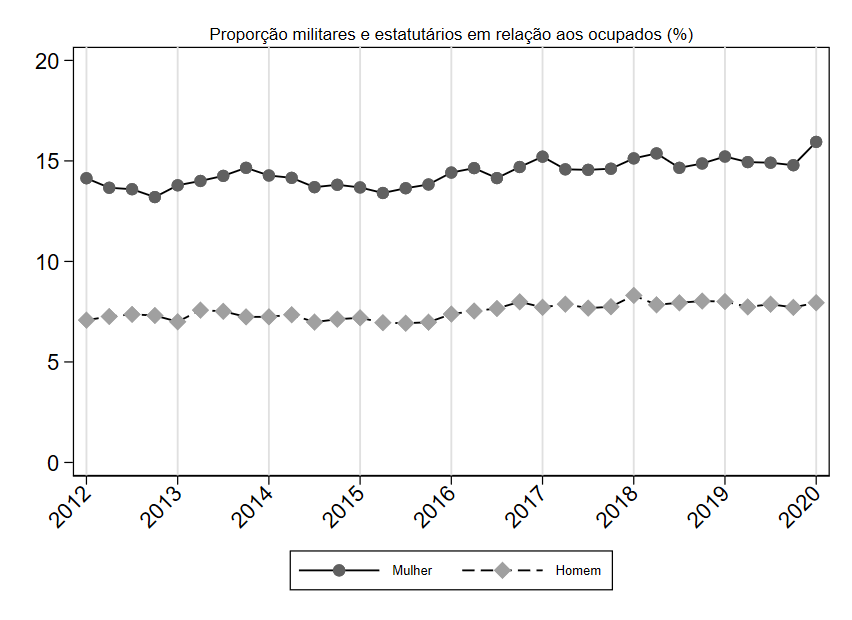
\includegraphics[width=1.0\linewidth]{../../analysis/output/composicao_demografica/genero/_composicao_demografica_genero_prop_militar.png}
  \caption{}
  \label{fig:_composicao_demografica_genero_prop_militar}
\end{figure}
\end{frame}


\begin{frame}[label=_composicao_demografica_genero_prop_empregadoSC]{}
\textit{\hyperlink{_composicao_demografica_genero}{\beamerbutton{Voltar}}}
\begin{figure}
  \centering
  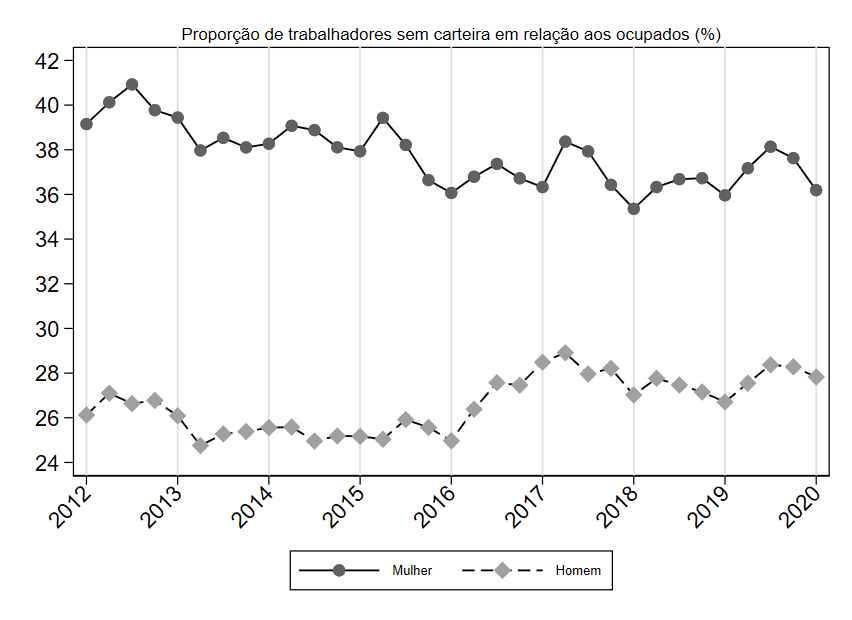
\includegraphics[width=1.0\linewidth]{../../analysis/output/composicao_demografica/genero/_composicao_demografica_genero_prop_empregadoSC.png}
  \caption{}
  \label{fig:_composicao_demografica_genero_prop_empregadoSC}
\end{figure}
\end{frame}

\begin{frame}[label=_composicao_demografica_genero_prop_empregadoCC]{}
\textit{\hyperlink{_composicao_demografica_genero}{\beamerbutton{Voltar}}}
\begin{figure}
  \centering
  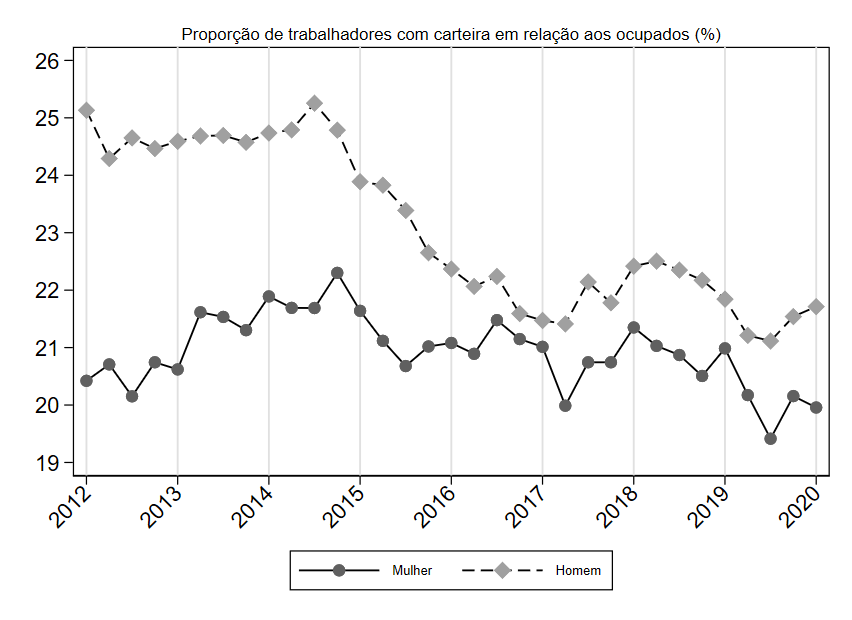
\includegraphics[width=1.0\linewidth]{../../analysis/output/composicao_demografica/genero/_composicao_demografica_genero_prop_empregadoCC.png}
  \caption{}
  \label{fig:_composicao_demografica_genero_prop_empregadoCC}
\end{figure}
\end{frame}

\begin{frame}[label=_composicao_demografica_genero_prop_empregador]{}
\textit{\hyperlink{_composicao_demografica_genero}{\beamerbutton{Voltar}}}
\begin{figure}
  \centering
  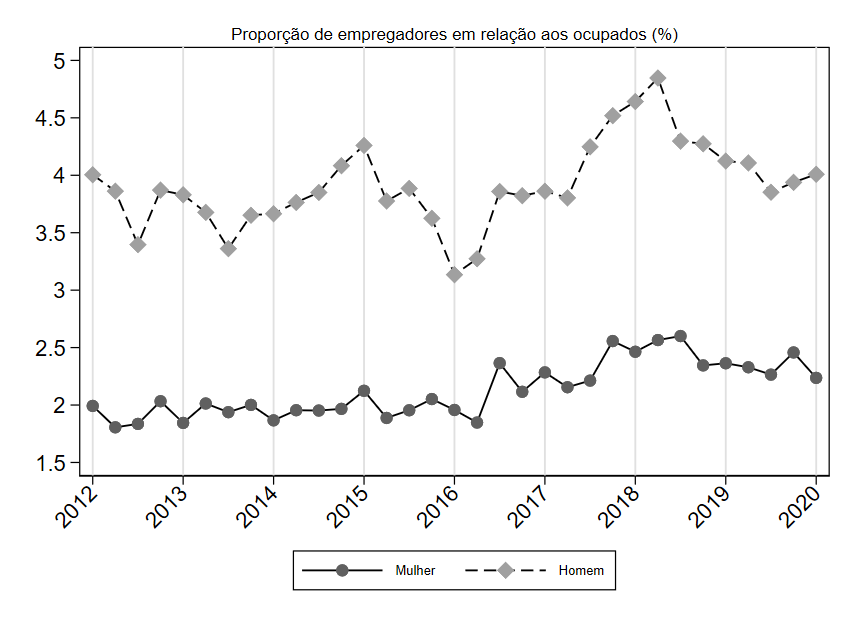
\includegraphics[width=1.0\linewidth]{../../analysis/output/composicao_demografica/genero/_composicao_demografica_genero_prop_empregador.png}
  \caption{}
  \label{fig:_composicao_demografica_genero_prop_empregador}
\end{figure}
\end{frame}



\begin{frame}[label=_composicao_demografica_genero_prop_cpropria]{}
\textit{\hyperlink{_composicao_demografica_genero}{\beamerbutton{Voltar}}}
\begin{figure}
  \centering
  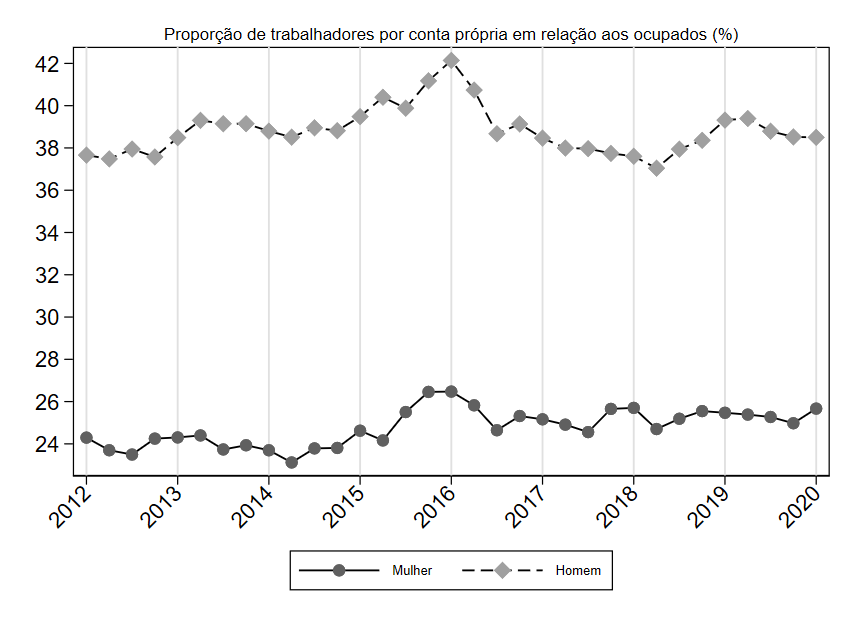
\includegraphics[width=1.0\linewidth]{../../analysis/output/composicao_demografica/genero/_composicao_demografica_genero_prop_cpropria.png}
  \caption{}
  \label{fig:_composicao_demografica_genero_prop_cpropria}
\end{figure}
\end{frame}

\begin{frame}[label=_composicao_demografica_genero_prop_cpropriaC]{}
\textit{\hyperlink{_composicao_demografica_genero}{\beamerbutton{Voltar}}}
\begin{figure}
  \centering
  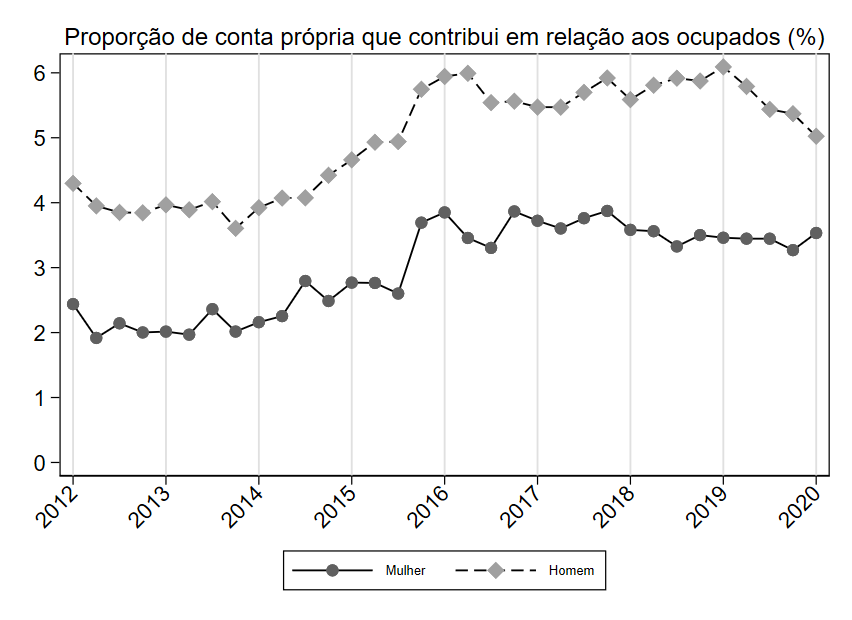
\includegraphics[width=1.0\linewidth]{../../analysis/output/composicao_demografica/genero/_composicao_demografica_genero_prop_cpropriaC.png}
  \caption{}
  \label{fig:_composicao_demografica_genero_prop_cpropriaC}
\end{figure}
\end{frame}

\begin{frame}[label=_composicao_demografica_genero_prop_cpropriaNc]{}
\textit{\hyperlink{_composicao_demografica_genero}{\beamerbutton{Voltar}}}
\begin{figure}
  \centering
  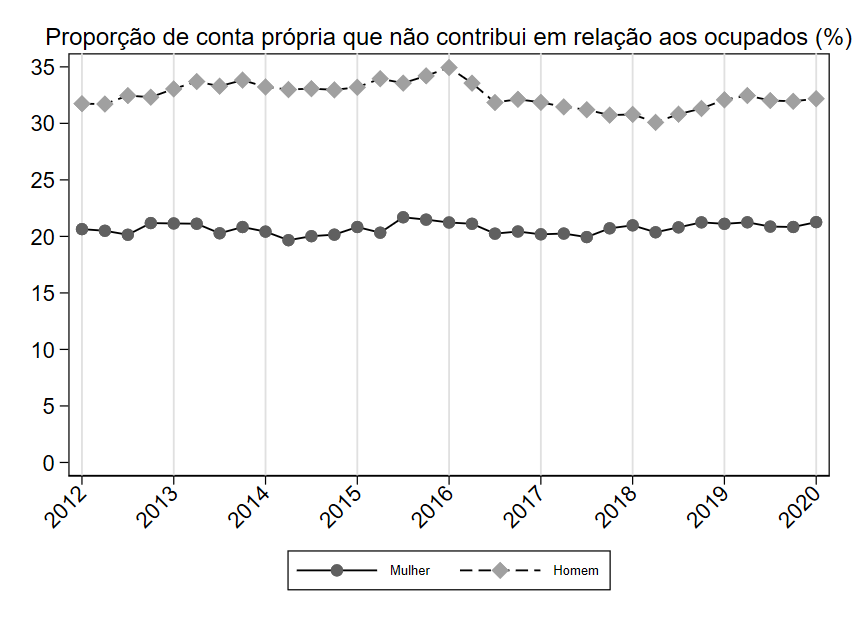
\includegraphics[width=1.0\linewidth]{../../analysis/output/composicao_demografica/genero/_composicao_demografica_genero_prop_cpropriaNc.png}
  \caption{}
  \label{fig:_composicao_demografica_genero_prop_cpropriaNc}
\end{figure}
\end{frame}
\begin{frame}[label=_composicao_demografica_faixa_etaria]{Composição Demográfica: Faixa Etária}
{\footnotesize Fonte de dados: Dados da PNAD Contínua Trimestral (2012-2020)}
\begin{itemize}
\item{Taxa de ocupação: \hyperlink{_composicao_demografica_faixa_etaria_taxa_de_ocupacao}{\beamerbutton{clique aqui}}}
\item{Taxa de informalidade: \hyperlink{_composicao_demografica_faixa_etaria_taxa_de_informalidade}{\beamerbutton{clique aqui}}}
\item{Taxa de desemprego: \hyperlink{_composicao_demografica_faixa_etaria_taxa_de_desemprego}{\beamerbutton{clique aqui}}}
\item{Proporção de militares e estatutários: \hyperlink{_composicao_demografica_faixa_etaria_prop_militar}{\beamerbutton{clique aqui}}}
\item{Proporção de empregados sem carteira: \hyperlink{_composicao_demografica_faixa_etaria_prop_empregadoSC}{\beamerbutton{clique aqui}}}
\item{Proporção de empregados com carteira: \hyperlink{_composicao_demografica_faixa_etaria_prop_empregadoCC}{\beamerbutton{clique aqui}}}
\item{Proporção de empregadores \hyperlink{_composicao_demografica_faixa_etaria_prop_empregador}{\beamerbutton{clique aqui}}}
\item{Proporção de conta própria: \hyperlink{_composicao_demografica_faixa_etaria_prop_cpropria}{\beamerbutton{clique aqui}}}
\item{Proporção de conta própria que contribui: \hyperlink{_composicao_demografica_faixa_etaria_prop_cpropriaC}{\beamerbutton{clique aqui}}}
\item{Proporção de conta própria que não contribui: \hyperlink{_composicao_demografica_faixa_etaria_prop_cpropriaNc}{\beamerbutton{clique aqui}}}
\end{itemize}

\begin{small}
\textit{Retornar ao índice principal da composição demográfica: \hyperlink{_composicao_demografica}{\beamerbutton{AQUI}} }
\end{small}

\end{frame}

\begin{frame}[label=_composicao_demografica_faixa_etaria_taxa_de_ocupacao]{}
\textit{\hyperlink{_composicao_demografica_faixa_etaria}{\beamerbutton{Voltar}}}
\begin{figure}
  \centering
  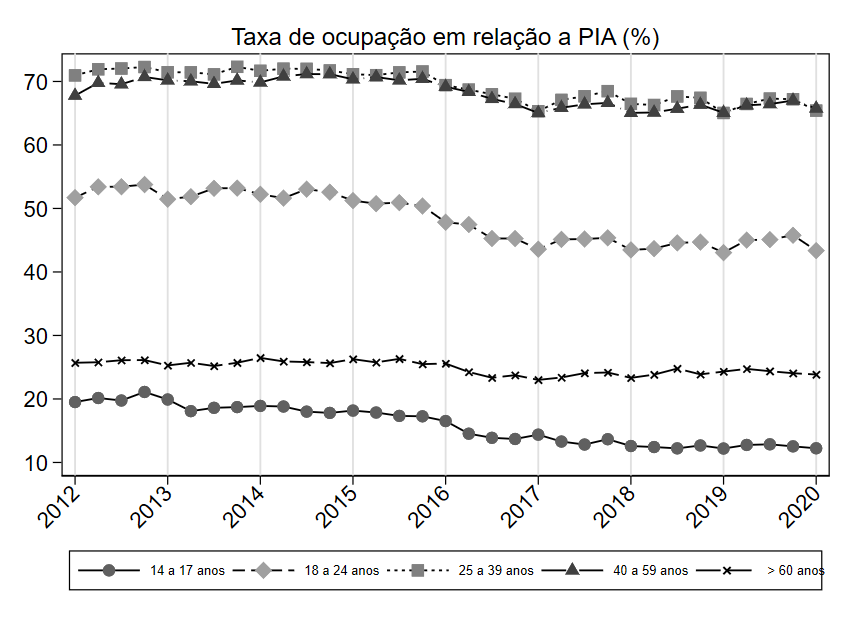
\includegraphics[width=1\linewidth]{../../analysis/output/composicao_demografica/faixa_etaria/_composicao_demografica_faixa_etaria_taxa_de_ocupacao.png}
  \caption{}
  \label{fig:_composicao_demografica_faixa_etaria_taxa_de_ocupacao}
\end{figure}
\end{frame}

\begin{frame}[label=_composicao_demografica_faixa_etaria_taxa_de_informalidade]{}
\textit{\hyperlink{_composicao_demografica_faixa_etaria}{\beamerbutton{Voltar}}}
\begin{figure}
  \centering
  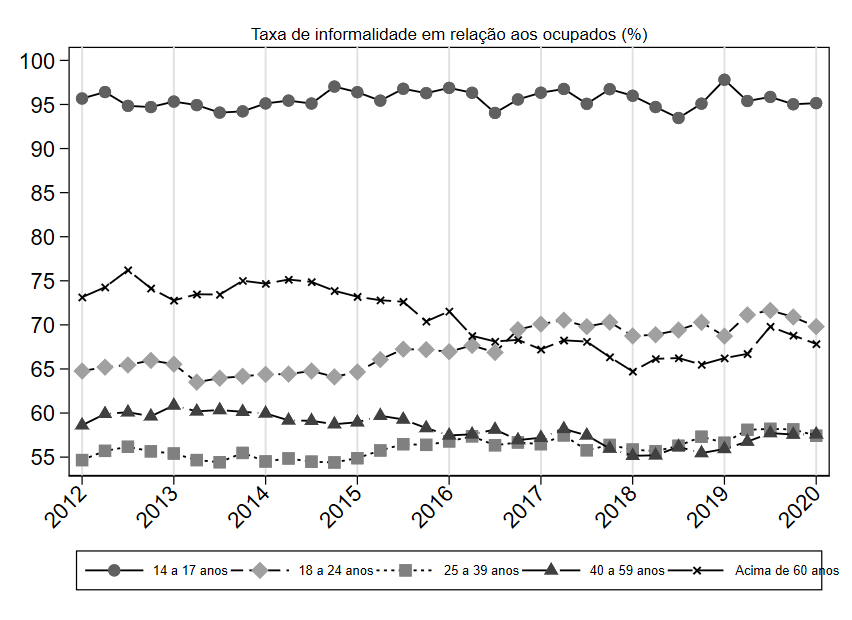
\includegraphics[width=1.0\linewidth]{../../analysis/output/composicao_demografica/faixa_etaria/_composicao_demografica_faixa_etaria_taxa_de_informalidade.png}
  \caption{}
  \label{fig:_composicao_demografica_faixa_etaria_taxa_de_informalidade}
\end{figure}
\end{frame}

\begin{frame}[label=_composicao_demografica_faixa_etaria_taxa_de_desemprego]{}
\textit{\hyperlink{_composicao_demografica_faixa_etaria}{\beamerbutton{Voltar}}}
\begin{figure}
  \centering
  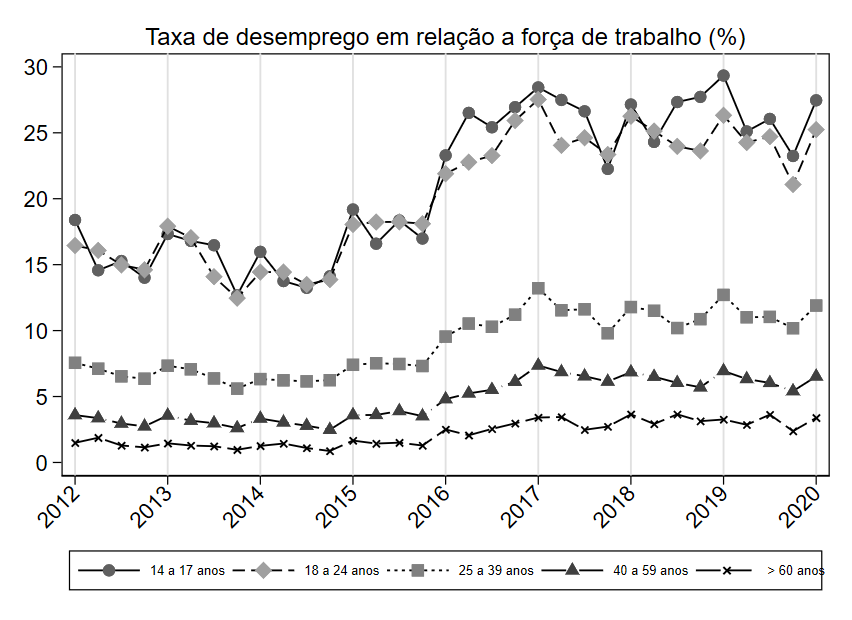
\includegraphics[width=1.0\linewidth]{../../analysis/output/composicao_demografica/faixa_etaria/_composicao_demografica_faixa_etaria_taxa_de_desemprego.png}
  \caption{}
  \label{fig:_composicao_demografica_faixa_etaria_taxa_de_desemprego}
\end{figure}
\end{frame}

\begin{frame}[label=_composicao_demografica_faixa_etaria_prop_militar]{}
\textit{\hyperlink{_composicao_demografica_faixa_etaria}{\beamerbutton{Voltar}}}
\begin{figure}
  \centering
  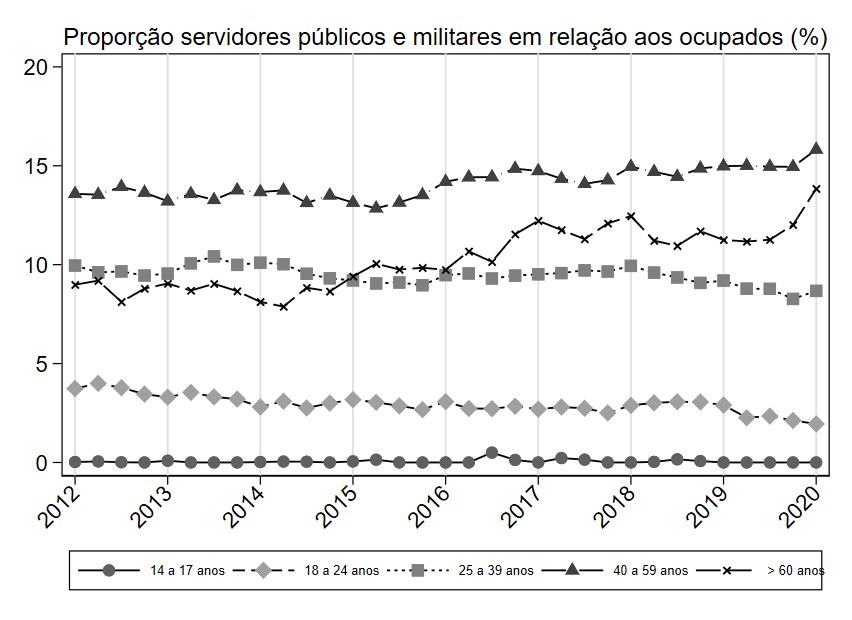
\includegraphics[width=1.0\linewidth]{../../analysis/output/composicao_demografica/faixa_etaria/_composicao_demografica_faixa_etaria_prop_militar.png}
  \caption{}
  \label{fig:_composicao_demografica_faixa_etaria_prop_militar}
\end{figure}
\end{frame}


\begin{frame}[label=_composicao_demografica_faixa_etaria_prop_empregadoSC]{}
\textit{\hyperlink{_composicao_demografica_faixa_etaria}{\beamerbutton{Voltar}}}
\begin{figure}
  \centering
  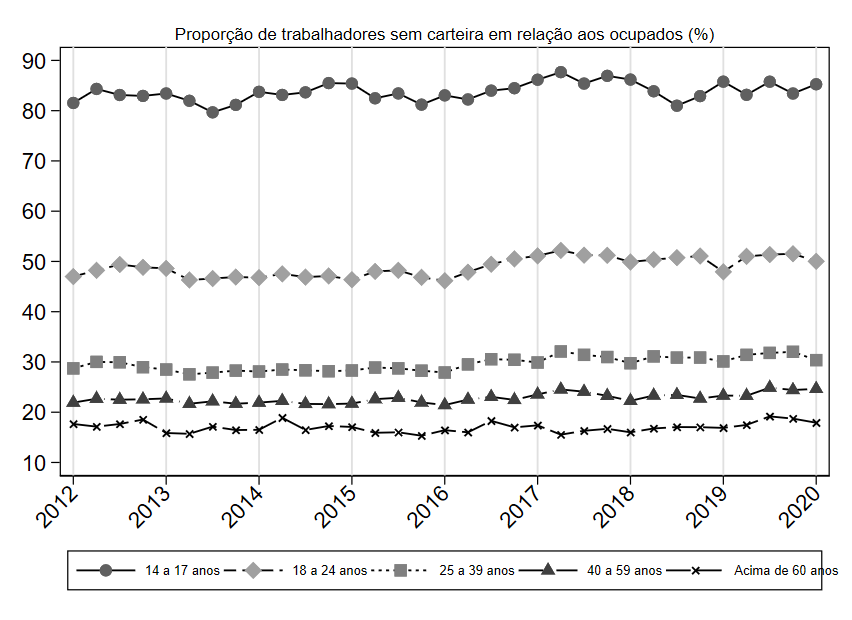
\includegraphics[width=1.0\linewidth]{../../analysis/output/composicao_demografica/faixa_etaria/_composicao_demografica_faixa_etaria_prop_empregadoSC.png}
  \caption{}
  \label{fig:_composicao_demografica_faixa_etaria_prop_empregadoSC}
\end{figure}
\end{frame}

\begin{frame}[label=_composicao_demografica_faixa_etaria_prop_empregadoCC]{}
\textit{\hyperlink{_composicao_demografica_faixa_etaria}{\beamerbutton{Voltar}}}
\begin{figure}
  \centering
  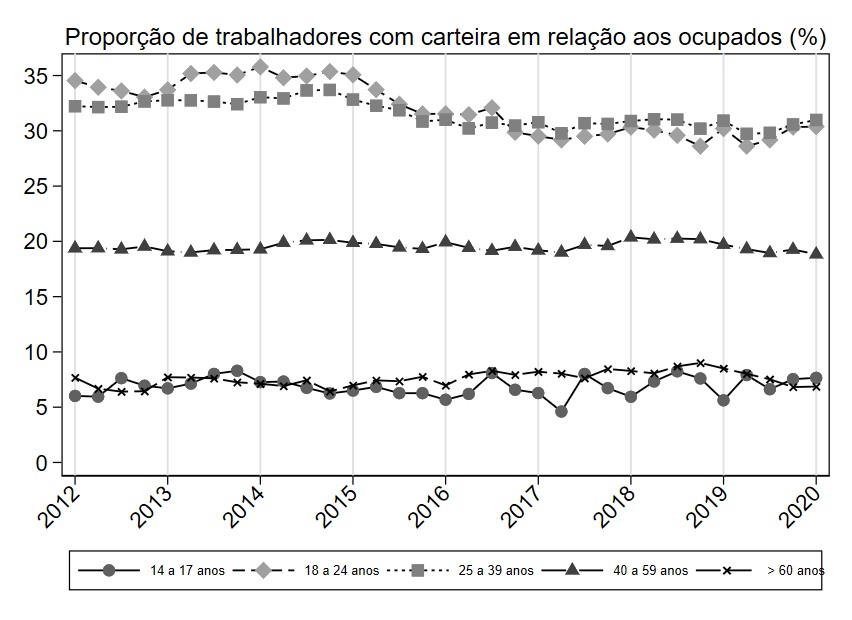
\includegraphics[width=1.0\linewidth]{../../analysis/output/composicao_demografica/faixa_etaria/_composicao_demografica_faixa_etaria_prop_empregadoCC.png}
  \caption{}
  \label{fig:_composicao_demografica_faixa_etaria_prop_empregadoCC}
\end{figure}
\end{frame}

\begin{frame}[label=_composicao_demografica_faixa_etaria_prop_empregador]{}
\textit{\hyperlink{_composicao_demografica_faixa_etaria}{\beamerbutton{Voltar}}}
\begin{figure}
  \centering
  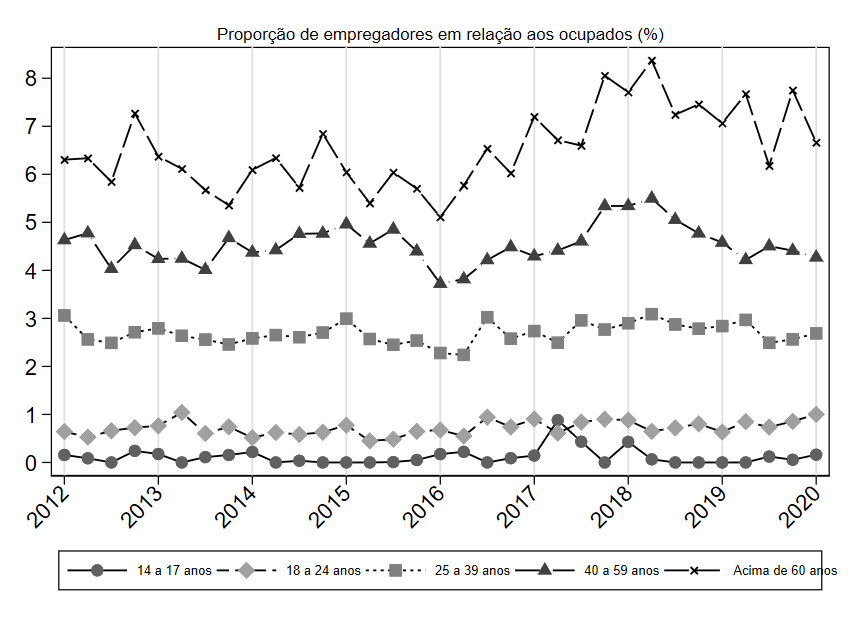
\includegraphics[width=1.0\linewidth]{../../analysis/output/composicao_demografica/faixa_etaria/_composicao_demografica_faixa_etaria_prop_empregador.png}
  \caption{}
  \label{fig:_composicao_demografica_faixa_etaria_prop_empregador}
\end{figure}
\end{frame}



\begin{frame}[label=_composicao_demografica_faixa_etaria_prop_cpropria]{}
\textit{\hyperlink{_composicao_demografica_faixa_etaria}{\beamerbutton{Voltar}}}
\begin{figure}
  \centering
  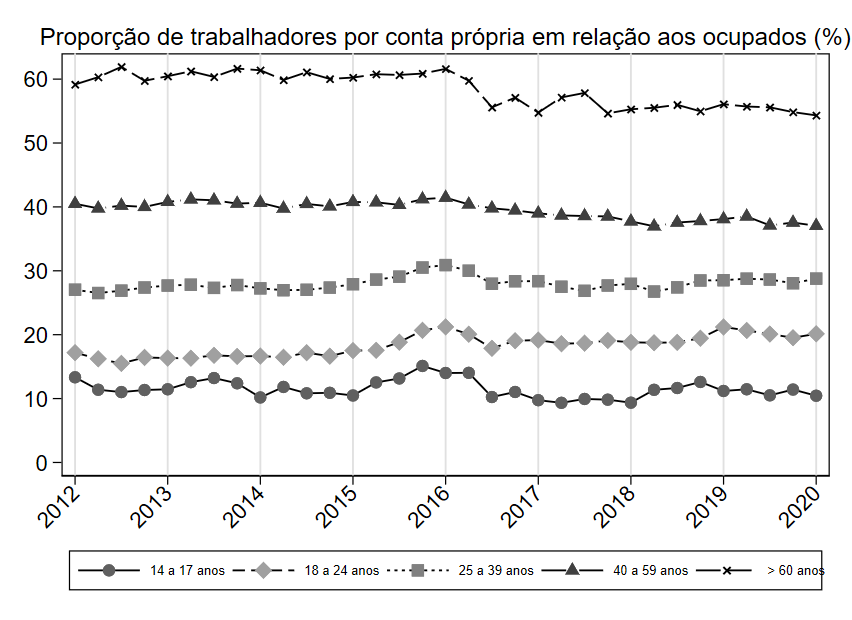
\includegraphics[width=1.0\linewidth]{../../analysis/output/composicao_demografica/faixa_etaria/_composicao_demografica_faixa_etaria_prop_cpropria.png}
  \caption{}
  \label{fig:_composicao_demografica_faixa_etaria_prop_cpropria}
\end{figure}
\end{frame}

\begin{frame}[label=_composicao_demografica_faixa_etaria_prop_cpropriaC]{}
\textit{\hyperlink{_composicao_demografica_faixa_etaria}{\beamerbutton{Voltar}}}
\begin{figure}
  \centering
  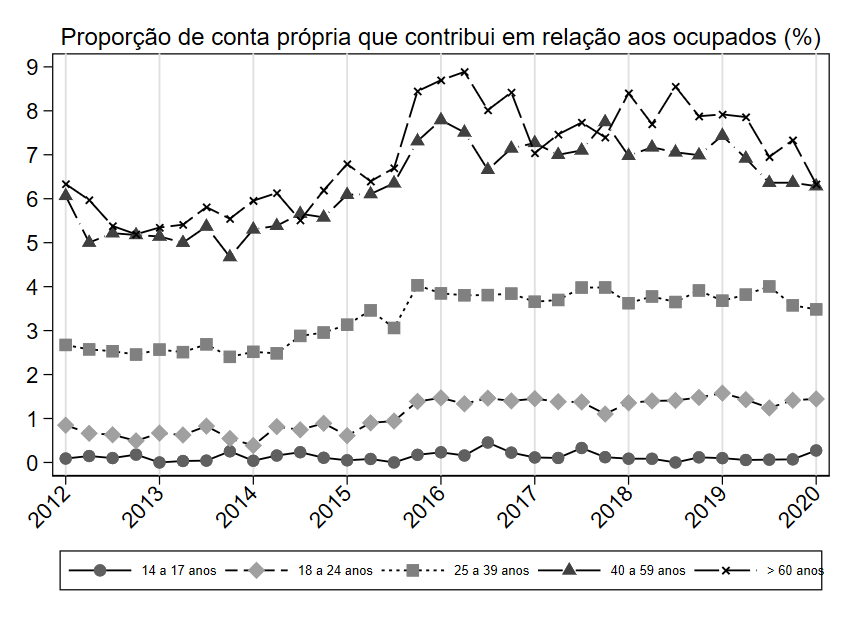
\includegraphics[width=1.0\linewidth]{../../analysis/output/composicao_demografica/faixa_etaria/_composicao_demografica_faixa_etaria_prop_cpropriaC.png}
  \caption{}
  \label{fig:_composicao_demografica_faixa_etaria_prop_cpropriaC}
\end{figure}
\end{frame}

\begin{frame}[label=_composicao_demografica_faixa_etaria_prop_cpropriaNc]{}
\textit{\hyperlink{_composicao_demografica_faixa_etaria}{\beamerbutton{Voltar}}}
\begin{figure}
  \centering
  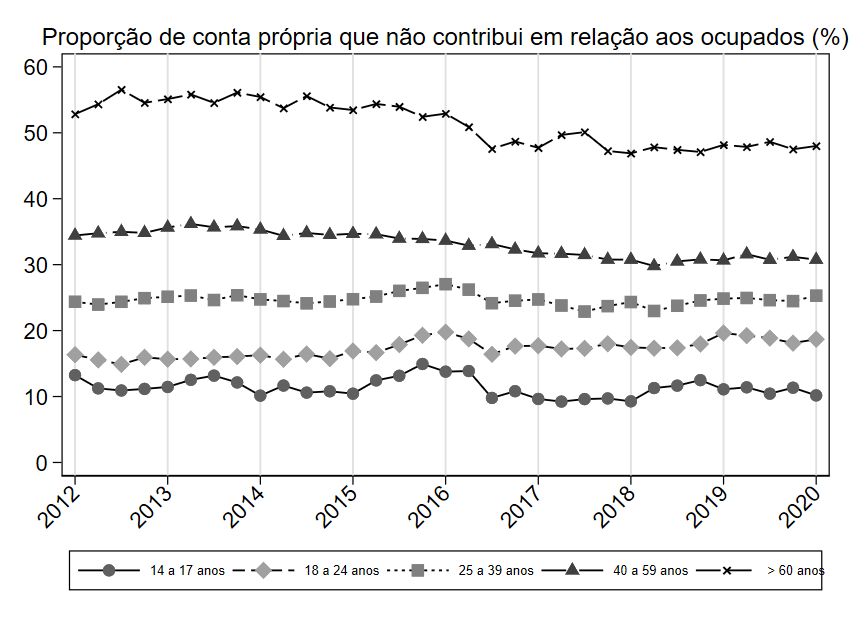
\includegraphics[width=1.0\linewidth]{../../analysis/output/composicao_demografica/faixa_etaria/_composicao_demografica_faixa_etaria_prop_cpropriaNc.png}
  \caption{}
  \label{fig:_composicao_demografica_faixa_etaria_prop_cpropriaNc}
\end{figure}
\end{frame}
\begin{frame}[label=_composicao_demografica_educacao]{Composição Demográfica: Educação}
{\footnotesize Fonte de dados: Dados da PNAD Contínua Trimestral (2012-2020)}
\begin{itemize}
\item{Taxa de ocupação: \hyperlink{_composicao_demografica_educacao_taxa_de_ocupacao}{\beamerbutton{clique aqui}}}
\item{Taxa de informalidade: \hyperlink{_composicao_demografica_educacao_taxa_de_informalidade}{\beamerbutton{clique aqui}}}
\item{Taxa de desemprego: \hyperlink{_composicao_demografica_educacao_taxa_de_desemprego}{\beamerbutton{clique aqui}}}
\item{Taxa de participação: \hyperlink{_composicao_demografica_educacao_taxa_de_participacao}{\beamerbutton{clique aqui}}}
\item{Proporção de servidores públicos e militares: \hyperlink{_composicao_demografica_educacao_prop_militar}{\beamerbutton{clique aqui}}}
\item{Proporção de empregados sem carteira: \hyperlink{_composicao_demografica_educacao_prop_empregadoSC}{\beamerbutton{clique aqui}}}
\item{Proporção de empregados com carteira: \hyperlink{_composicao_demografica_educacao_prop_empregadoCC}{\beamerbutton{clique aqui}}}
\item{Proporção de empregadores \hyperlink{_composicao_demografica_educacao_prop_empregador}{\beamerbutton{clique aqui}}}
\item{Proporção de conta própria: \hyperlink{_composicao_demografica_educacao_prop_cpropria}{\beamerbutton{clique aqui}}}
\item{Proporção de conta própria que contribui: \hyperlink{_composicao_demografica_educacao_prop_cpropriaC}{\beamerbutton{clique aqui}}}
\item{Proporção de conta própria que não contribui: \hyperlink{_composicao_demografica_educacao_prop_cpropriaNc}{\beamerbutton{clique aqui}}}
\end{itemize}

\begin{small}
\textit{Retornar ao índice principal da composição demográfica: \hyperlink{_composicao_demografica}{\beamerbutton{AQUI}} }
\end{small}

\end{frame}

\begin{frame}[label=_composicao_demografica_educacao_taxa_de_ocupacao]{}
\textit{\hyperlink{_composicao_demografica_educacao}{\beamerbutton{Voltar}}}
\begin{figure}
  \centering
  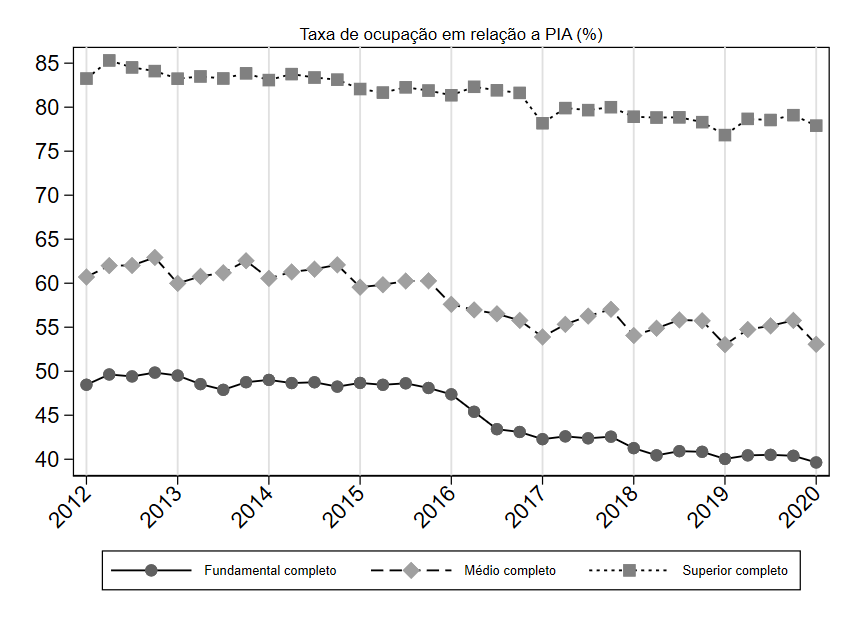
\includegraphics[width=1\linewidth]{../../analysis/output/composicao_demografica/educacao/_composicao_demografica_educacao_taxa_de_ocupacao.png}
  \caption{}
  \label{fig:_composicao_demografica_educacao_taxa_de_ocupacao}
\end{figure}
\end{frame}

\begin{frame}[label=_composicao_demografica_educacao_taxa_de_informalidade]{}
\textit{\hyperlink{_composicao_demografica_educacao}{\beamerbutton{Voltar}}}
\begin{figure}
  \centering
  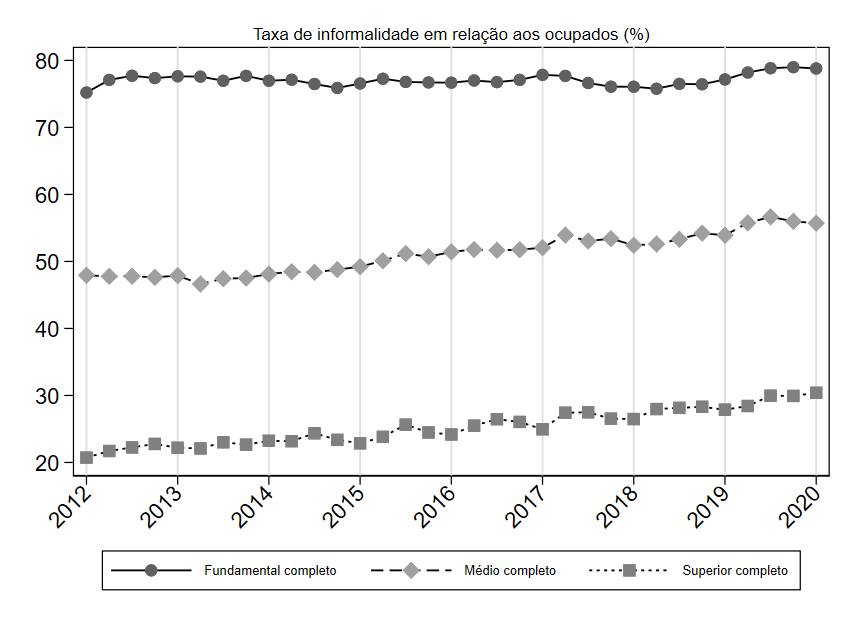
\includegraphics[width=1.0\linewidth]{../../analysis/output/composicao_demografica/educacao/_composicao_demografica_educacao_taxa_de_informalidade.png}
  \caption{}
  \label{fig:_composicao_demografica_educacao_taxa_de_informalidade}
\end{figure}
\end{frame}

\begin{frame}[label=_composicao_demografica_educacao_taxa_de_desemprego]{}
\textit{\hyperlink{_composicao_demografica_educacao}{\beamerbutton{Voltar}}}
\begin{figure}
  \centering
  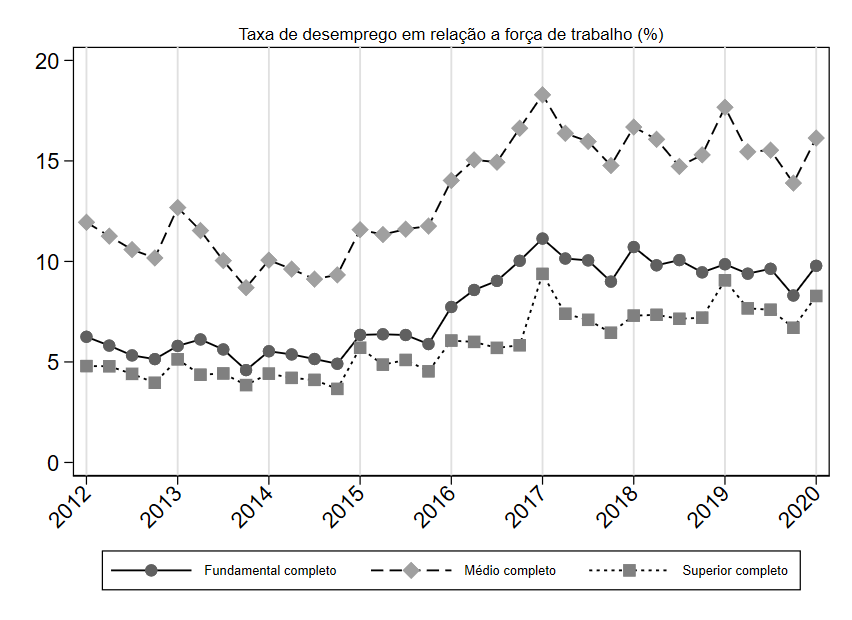
\includegraphics[width=1.0\linewidth]{../../analysis/output/composicao_demografica/educacao/_composicao_demografica_educacao_taxa_de_desemprego.png}
  \caption{}
  \label{fig:_composicao_demografica_educacao_taxa_de_desemprego}
\end{figure}
\end{frame}

\begin{frame}[label=_composicao_demografica_educacao_taxa_de_participacao]{}
\textit{\hyperlink{_composicao_demografica_educacao}{\beamerbutton{Voltar}}}
\begin{figure}
  \centering
  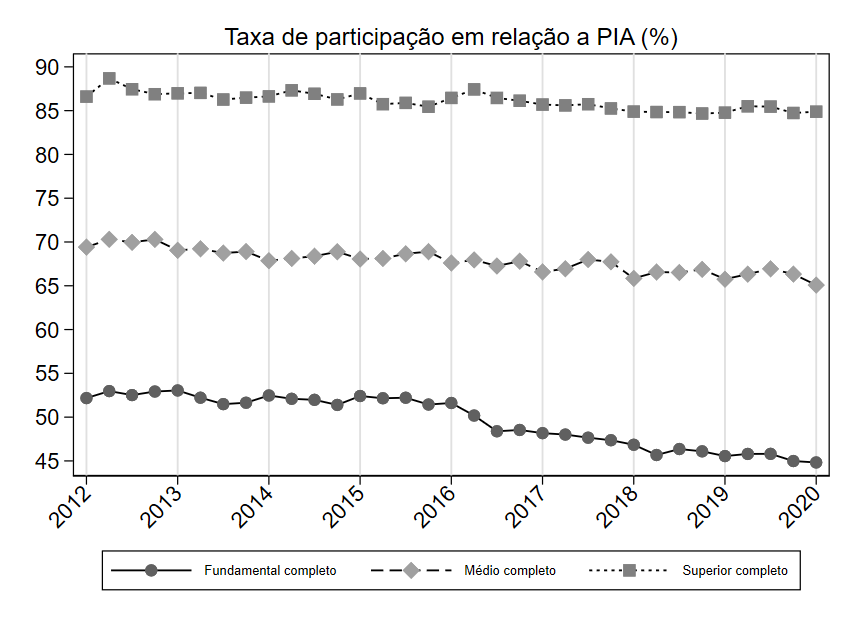
\includegraphics[width=1.0\linewidth]{../../analysis/output/composicao_demografica/educacao/_composicao_demografica_educacao_taxa_de_participacao.png}
  \caption{}
  \label{fig:_composicao_demografica_educacao_taxa_de_participacao}
\end{figure}
\end{frame}

\begin{frame}[label=_composicao_demografica_educacao_prop_militar]{}
\textit{\hyperlink{_composicao_demografica_educacao}{\beamerbutton{Voltar}}}
\begin{figure}
  \centering
  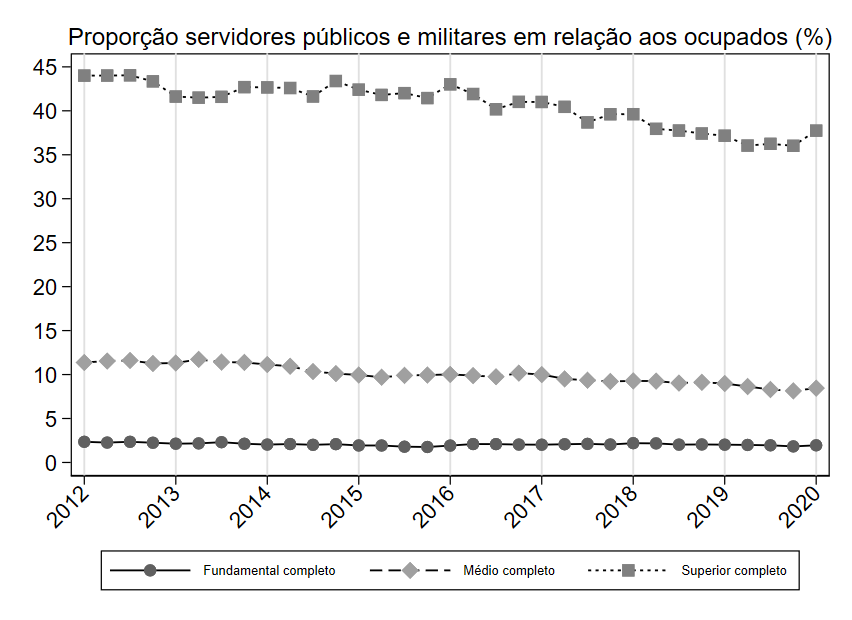
\includegraphics[width=1.0\linewidth]{../../analysis/output/composicao_demografica/educacao/_composicao_demografica_educacao_prop_militar.png}
  \caption{}
  \label{fig:_composicao_demografica_educacao_prop_militar}
\end{figure}
\end{frame}


\begin{frame}[label=_composicao_demografica_educacao_prop_empregadoSC]{}
\textit{\hyperlink{_composicao_demografica_educacao}{\beamerbutton{Voltar}}}
\begin{figure}
  \centering
  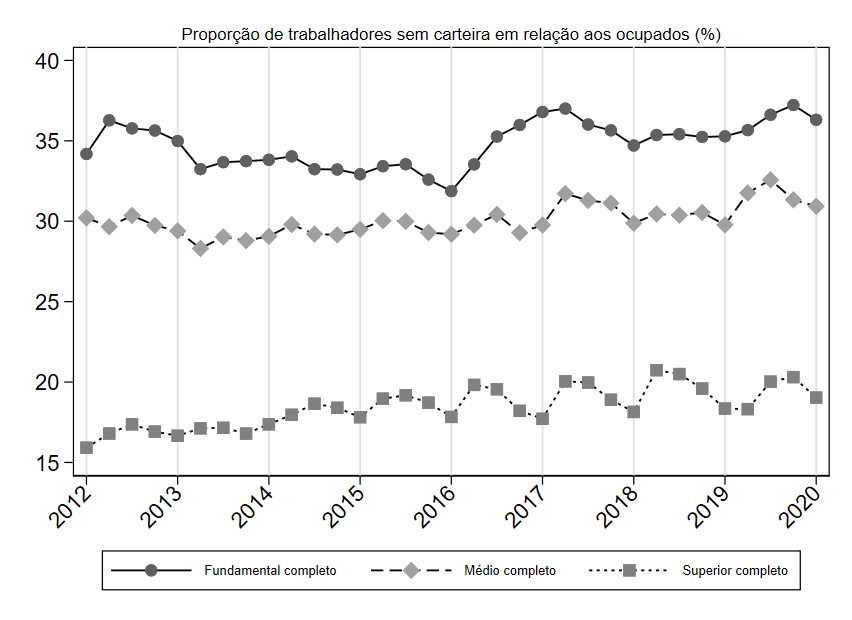
\includegraphics[width=1.0\linewidth]{../../analysis/output/composicao_demografica/educacao/_composicao_demografica_educacao_prop_empregadoSC.png}
  \caption{}
  \label{fig:_composicao_demografica_educacao_prop_empregadoSC}
\end{figure}
\end{frame}

\begin{frame}[label=_composicao_demografica_educacao_prop_empregadoCC]{}
\textit{\hyperlink{_composicao_demografica_educacao}{\beamerbutton{Voltar}}}
\begin{figure}
  \centering
  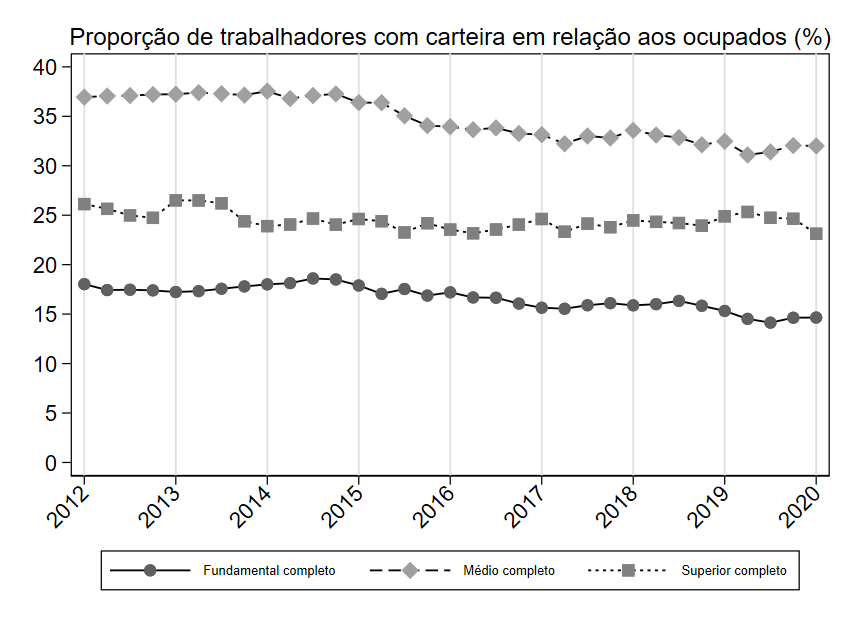
\includegraphics[width=1.0\linewidth]{../../analysis/output/composicao_demografica/educacao/_composicao_demografica_educacao_prop_empregadoCC.png}
  \caption{}
  \label{fig:_composicao_demografica_educacao_prop_empregadoCC}
\end{figure}
\end{frame}

\begin{frame}[label=_composicao_demografica_educacao_prop_empregador]{}
\textit{\hyperlink{_composicao_demografica_educacao}{\beamerbutton{Voltar}}}
\begin{figure}
  \centering
  \includegraphics[width=1.0\linewidth]{../../analysis/output/composicao_demografica/educacao/_composicao_demografica_educacao_prop_empregador.png}
  \caption{}
  \label{fig:_composicao_demografica_educacao_prop_empregador}
\end{figure}
\end{frame}



\begin{frame}[label=_composicao_demografica_educacao_prop_cpropria]{}
\textit{\hyperlink{_composicao_demografica_educacao}{\beamerbutton{Voltar}}}
\begin{figure}
  \centering
  \includegraphics[width=1.0\linewidth]{../../analysis/output/composicao_demografica/educacao/_composicao_demografica_educacao_prop_cpropria.png}
  \caption{}
  \label{fig:_composicao_demografica_educacao_prop_cpropria}
\end{figure}
\end{frame}

\begin{frame}[label=_composicao_demografica_educacao_prop_cpropriaC]{}
\textit{\hyperlink{_composicao_demografica_educacao}{\beamerbutton{Voltar}}}
\begin{figure}
  \centering
  \includegraphics[width=1.0\linewidth]{../../analysis/output/composicao_demografica/educacao/_composicao_demografica_educacao_prop_cpropriaC.png}
  \caption{}
  \label{fig:_composicao_demografica_educacao_prop_cpropriaC}
\end{figure}
\end{frame}

\begin{frame}[label=_composicao_demografica_educacao_prop_cpropriaNc]{}
\textit{\hyperlink{_composicao_demografica_educacao}{\beamerbutton{Voltar}}}
\begin{figure}
  \centering
  \includegraphics[width=1.0\linewidth]{../../analysis/output/composicao_demografica/educacao/_composicao_demografica_educacao_prop_cpropriaNc.png}
  \caption{}
  \label{fig:_composicao_demografica_educacao_prop_cpropriaNc}
\end{figure}
\end{frame}
\begin{frame}[label=_composicao_demografica_setor]{Composição Demográfica: Setor Ocupacional}
{\footnotesize Fonte de dados: Dados da PNAD Contínua Trimestral (2012-2020)}
\begin{itemize}
\item{Taxa de informalidade: \hyperlink{_composicao_demografica_setor_taxa_de_informalidade}{\beamerbutton{clique aqui}}}
\item{Proporção deservidores públicos e militares: \hyperlink{_composicao_demografica_setor_prop_militar}{\beamerbutton{clique aqui}}}
\item{Proporção de empregados sem carteira: \hyperlink{_composicao_demografica_setor_prop_empregadoSC}{\beamerbutton{clique aqui}}}
\item{Proporção de empregados com carteira: \hyperlink{_composicao_demografica_setor_prop_empregadoCC}{\beamerbutton{clique aqui}}}
\item{Proporção de empregadores \hyperlink{_composicao_demografica_setor_prop_empregador}{\beamerbutton{clique aqui}}}
\item{Proporção de conta própria: \hyperlink{_composicao_demografica_setor_prop_cpropria}{\beamerbutton{clique aqui}}}
\item{Proporção de conta própria que contribui: \hyperlink{_composicao_demografica_setor_prop_cpropriaC}{\beamerbutton{clique aqui}}}
\item{Proporção de conta própria que não contribui: \hyperlink{_composicao_demografica_setor_prop_cpropriaNc}{\beamerbutton{clique aqui}}}
\end{itemize}

\begin{small}
\textit{Retornar ao índice principal da composição demográfica: \hyperlink{_composicao_demografica}{\beamerbutton{AQUI}} }
\end{small}

\end{frame}


\begin{frame}[label=_composicao_demografica_setor_taxa_de_informalidade]{}
\textit{\hyperlink{_composicao_demografica_setor}{\beamerbutton{Voltar}}}
\begin{figure}
  \centering
  \includegraphics[width=1.0\linewidth]{../../analysis/output/composicao_demografica/setor/_composicao_demografica_setor_taxa_de_informalidade.png}
  \caption{}
  \label{fig:_composicao_demografica_setor_taxa_de_informalidade}
\end{figure}
\end{frame}


\begin{frame}[label=_composicao_demografica_setor_prop_militar]{}
\textit{\hyperlink{_composicao_demografica_setor}{\beamerbutton{Voltar}}}
\begin{figure}
  \centering
  \includegraphics[width=1.0\linewidth]{../../analysis/output/composicao_demografica/setor/_composicao_demografica_setor_prop_militar.png}
  \caption{}
  \label{fig:_composicao_demografica_setor_prop_militar}
\end{figure}
\end{frame}


\begin{frame}[label=_composicao_demografica_setor_prop_empregadoSC]{}
\textit{\hyperlink{_composicao_demografica_setor}{\beamerbutton{Voltar}}}
\begin{figure}
  \centering
  \includegraphics[width=1.0\linewidth]{../../analysis/output/composicao_demografica/setor/_composicao_demografica_setor_prop_empregadoSC.png}
  \caption{}
  \label{fig:_composicao_demografica_setor_prop_empregadoSC}
\end{figure}
\end{frame}

\begin{frame}[label=_composicao_demografica_setor_prop_empregadoCC]{}
\textit{\hyperlink{_composicao_demografica_setor}{\beamerbutton{Voltar}}}
\begin{figure}
  \centering
  \includegraphics[width=1.0\linewidth]{../../analysis/output/composicao_demografica/setor/_composicao_demografica_setor_prop_empregadoCC.png}
  \caption{}
  \label{fig:_composicao_demografica_setor_prop_empregadoCC}
\end{figure}
\end{frame}

\begin{frame}[label=_composicao_demografica_setor_prop_empregador]{}
\textit{\hyperlink{_composicao_demografica_setor}{\beamerbutton{Voltar}}}
\begin{figure}
  \centering
  \includegraphics[width=1.0\linewidth]{../../analysis/output/composicao_demografica/setor/_composicao_demografica_setor_prop_empregador.png}
  \caption{}
  \label{fig:_composicao_demografica_setor_prop_empregador}
\end{figure}
\end{frame}



\begin{frame}[label=_composicao_demografica_setor_prop_cpropria]{}
\textit{\hyperlink{_composicao_demografica_setor}{\beamerbutton{Voltar}}}
\begin{figure}
  \centering
  \includegraphics[width=1.0\linewidth]{../../analysis/output/composicao_demografica/setor/_composicao_demografica_setor_prop_cpropria.png}
  \caption{}
  \label{fig:_composicao_demografica_setor_prop_cpropria}
\end{figure}
\end{frame}

\begin{frame}[label=_composicao_demografica_setor_prop_cpropriaC]{}
\textit{\hyperlink{_composicao_demografica_setor}{\beamerbutton{Voltar}}}
\begin{figure}
  \centering
  \includegraphics[width=1.0\linewidth]{../../analysis/output/composicao_demografica/setor/_composicao_demografica_setor_prop_cpropriaC.png}
  \caption{}
  \label{fig:_composicao_demografica_setor_prop_cpropriaC}
\end{figure}
\end{frame}

\begin{frame}[label=_composicao_demografica_setor_prop_cpropriaNc]{}
\textit{\hyperlink{_composicao_demografica_setor}{\beamerbutton{Voltar}}}
\begin{figure}
  \centering
  \includegraphics[width=1.0\linewidth]{../../analysis/output/composicao_demografica/setor/_composicao_demografica_setor_prop_cpropriaNc.png}
  \caption{}
  \label{fig:_composicao_demografica_setor_prop_cpropriaNc}
\end{figure}
\end{frame}
\begin{frame}[label=_composicao_demografica_regiao_metro]{Composição Demográfica: Regiões metropolitanas}
{\footnotesize Fonte de dados: Dados da PNAD Contínua Trimestral (2012-2020)}
\begin{itemize}
\item{Taxa de ocupação: \hyperlink{_composicao_demografica_regiao_metro_taxa_de_ocupacao}{\beamerbutton{clique aqui}}}
\item{Taxa de informalidade: \hyperlink{_composicao_demografica_regiao_metro_taxa_de_informalidade}{\beamerbutton{clique aqui}}}
\item{Taxa de desemprego: \hyperlink{_composicao_demografica_regiao_metro_taxa_de_desemprego}{\beamerbutton{clique aqui}}}
\item{Taxa de participação: \hyperlink{_composicao_demografica_regiao_metro_taxa_de_participacao}{\beamerbutton{clique aqui}}}
\item{Proporção de servidores públicos e militares: \hyperlink{_composicao_demografica_regiao_metro_prop_militar}{\beamerbutton{clique aqui}}}
\item{Proporção de empregados sem carteira: \hyperlink{_composicao_demografica_regiao_metro_prop_empregadoSC}{\beamerbutton{clique aqui}}}
\item{Proporção de empregados com carteira: \hyperlink{_composicao_demografica_regiao_metro_prop_empregadoCC}{\beamerbutton{clique aqui}}}
\item{Proporção de empregadores \hyperlink{_composicao_demografica_regiao_metro_prop_empregador}{\beamerbutton{clique aqui}}}
\item{Proporção de conta própria: \hyperlink{_composicao_demografica_regiao_metro_prop_cpropria}{\beamerbutton{clique aqui}}}
\item{Proporção de conta própria que contribui: \hyperlink{_composicao_demografica_regiao_metro_prop_cpropriaC}{\beamerbutton{clique aqui}}}
\item{Proporção de conta própria que não contribui: \hyperlink{_composicao_demografica_regiao_metro_prop_cpropriaNc}{\beamerbutton{clique aqui}}}
\end{itemize}

\begin{small}
\textit{Retornar ao índice principal da composição demográfica: \hyperlink{_composicao_demografica}{\beamerbutton{AQUI}} }
\end{small}

\end{frame}

\begin{frame}[label=_composicao_demografica_regiao_metro_taxa_de_ocupacao]{}
\textit{\hyperlink{_composicao_demografica_regiao_metro}{\beamerbutton{Voltar}}}
\begin{figure}
  \centering
  \includegraphics[width=1\linewidth]{../../analysis/output/composicao_demografica/area_geografica/_composicao_demografica_regiao_metro_taxa_de_ocupacao.png}
  \caption{}
  \label{fig:_composicao_demografica_regiao_metro_taxa_de_ocupacao}
\end{figure}
\end{frame}

\begin{frame}[label=_composicao_demografica_regiao_metro_taxa_de_informalidade]{}
\textit{\hyperlink{_composicao_demografica_regiao_metro}{\beamerbutton{Voltar}}}
\begin{figure}
  \centering
  \includegraphics[width=1.0\linewidth]{../../analysis/output/composicao_demografica/area_geografica/_composicao_demografica_regiao_metro_taxa_de_informalidade.png}
  \caption{}
  \label{fig:_composicao_demografica_regiao_metro_taxa_de_informalidade}
\end{figure}
\end{frame}

\begin{frame}[label=_composicao_demografica_regiao_metro_taxa_de_desemprego]{}
\textit{\hyperlink{_composicao_demografica_regiao_metro}{\beamerbutton{Voltar}}}
\begin{figure}
  \centering
  \includegraphics[width=1.0\linewidth]{../../analysis/output/composicao_demografica/area_geografica/_composicao_demografica_regiao_metro_taxa_de_desemprego.png}
  \caption{}
  \label{fig:_composicao_demografica_regiao_metro_taxa_de_desemprego}
\end{figure}
\end{frame}

\begin{frame}[label=_composicao_demografica_regiao_metro_taxa_de_participacao]{}
\textit{\hyperlink{_composicao_demografica_regiao_metro}{\beamerbutton{Voltar}}}
\begin{figure}
  \centering
  \includegraphics[width=1.0\linewidth]{../../analysis/output/composicao_demografica/area_geografica/_composicao_demografica_regiao_metro_taxa_de_participacao.png}
  \caption{}
  \label{fig:_composicao_demografica_regiao_metro_taxa_de_participacao}
\end{figure}
\end{frame}

\begin{frame}[label=_composicao_demografica_regiao_metro_prop_militar]{}
\textit{\hyperlink{_composicao_demografica_regiao_metro}{\beamerbutton{Voltar}}}
\begin{figure}
  \centering
  \includegraphics[width=1.0\linewidth]{../../analysis/output/composicao_demografica/area_geografica/_composicao_demografica_regiao_metro_prop_militar.png}
  \caption{}
  \label{fig:_composicao_demografica_regiao_metro_prop_militar}
\end{figure}
\end{frame}


\begin{frame}[label=_composicao_demografica_regiao_metro_prop_empregadoSC]{}
\textit{\hyperlink{_composicao_demografica_regiao_metro}{\beamerbutton{Voltar}}}
\begin{figure}
  \centering
  \includegraphics[width=1.0\linewidth]{../../analysis/output/composicao_demografica/area_geografica/_composicao_demografica_regiao_metro_prop_empregadoSC.png}
  \caption{}
  \label{fig:_composicao_demografica_regiao_metro_prop_empregadoSC}
\end{figure}
\end{frame}

\begin{frame}[label=_composicao_demografica_regiao_metro_prop_empregadoCC]{}
\textit{\hyperlink{_composicao_demografica_regiao_metro}{\beamerbutton{Voltar}}}
\begin{figure}
  \centering
  \includegraphics[width=1.0\linewidth]{../../analysis/output/composicao_demografica/area_geografica/_composicao_demografica_regiao_metro_prop_empregadoCC.png}
  \caption{}
  \label{fig:_composicao_demografica_regiao_metro_prop_empregadoCC}
\end{figure}
\end{frame}

\begin{frame}[label=_composicao_demografica_regiao_metro_prop_empregador]{}
\textit{\hyperlink{_composicao_demografica_regiao_metro}{\beamerbutton{Voltar}}}
\begin{figure}
  \centering
  \includegraphics[width=1.0\linewidth]{../../analysis/output/composicao_demografica/area_geografica/_composicao_demografica_regiao_metro_prop_empregador.png}
  \caption{}
  \label{fig:_composicao_demografica_regiao_metro_prop_empregador}
\end{figure}
\end{frame}



\begin{frame}[label=_composicao_demografica_regiao_metro_prop_cpropria]{}
\textit{\hyperlink{_composicao_demografica_regiao_metro}{\beamerbutton{Voltar}}}
\begin{figure}
  \centering
  \includegraphics[width=1.0\linewidth]{../../analysis/output/composicao_demografica/area_geografica/_composicao_demografica_regiao_metro_prop_cpropria.png}
  \caption{}
  \label{fig:_composicao_demografica_regiao_metro_prop_cpropria}
\end{figure}
\end{frame}

\begin{frame}[label=_composicao_demografica_regiao_metro_prop_cpropriaC]{}
\textit{\hyperlink{_composicao_demografica_regiao_metro}{\beamerbutton{Voltar}}}
\begin{figure}
  \centering
  \includegraphics[width=1.0\linewidth]{../../analysis/output/composicao_demografica/area_geografica/_composicao_demografica_regiao_metro_prop_cpropriaC.png}
  \caption{}
  \label{fig:_composicao_demografica_regiao_metro_prop_cpropriaC}
\end{figure}
\end{frame}

\begin{frame}[label=_composicao_demografica_regiao_metro_prop_cpropriaNc]{}
\textit{\hyperlink{_composicao_demografica_regiao_metro}{\beamerbutton{Voltar}}}
\begin{figure}
  \centering
  \includegraphics[width=1.0\linewidth]{../../analysis/output/composicao_demografica/area_geografica/_composicao_demografica_regiao_metro_prop_cpropriaNc.png}
  \caption{}
  \label{fig:_composicao_demografica_regiao_metro_prop_cpropriaNc}
\end{figure}
\end{frame}
\begin{frame}[label=_composicao_demografica_rural_urbano]{Composição Demográfica: Zona rural vs zona urbana}
{\footnotesize Fonte de dados: Dados da PNAD Contínua Trimestral (2012-2020)}
\begin{itemize}
\item{Taxa de ocupação: \hyperlink{_composicao_demografica_rural_urbano_taxa_de_ocupacao}{\beamerbutton{clique aqui}}}
\item{Taxa de informalidade: \hyperlink{_composicao_demografica_rural_urbano_taxa_de_informalidade}{\beamerbutton{clique aqui}}}
\item{Taxa de desemprego: \hyperlink{_composicao_demografica_rural_urbano_taxa_de_desemprego}{\beamerbutton{clique aqui}}}
\item{Taxa de participação: \hyperlink{_composicao_demografica_rural_urbano_taxa_de_participacao}{\beamerbutton{clique aqui}}}
\item{Proporção de militares e estatutários: \hyperlink{_composicao_demografica_rural_urbano_prop_militar}{\beamerbutton{clique aqui}}}
\item{Proporção de empregados sem carteira: \hyperlink{_composicao_demografica_rural_urbano_prop_empregadoSC}{\beamerbutton{clique aqui}}}
\item{Proporção de empregados com carteira: \hyperlink{_composicao_demografica_rural_urbano_prop_empregadoCC}{\beamerbutton{clique aqui}}}
\item{Proporção de empregadores \hyperlink{_composicao_demografica_rural_urbano_prop_empregador}{\beamerbutton{clique aqui}}}
\item{Proporção de conta própria: \hyperlink{_composicao_demografica_rural_urbano_prop_cpropria}{\beamerbutton{clique aqui}}}
\item{Proporção de conta própria que contribui: \hyperlink{_composicao_demografica_rural_urbano_prop_cpropriaC}{\beamerbutton{clique aqui}}}
\item{Proporção de conta própria que não contribui: \hyperlink{_composicao_demografica_rural_urbano_prop_cpropriaNc}{\beamerbutton{clique aqui}}}
\end{itemize}

\begin{small}
\textit{Retornar ao índice principal da composição demográfica: \hyperlink{_composicao_demografica}{\beamerbutton{AQUI}} }
\end{small}

\end{frame}

\begin{frame}[label=_composicao_demografica_rural_urbano_taxa_de_ocupacao]{}
\textit{\hyperlink{_composicao_demografica_rural_urbano}{\beamerbutton{Voltar}}}
\begin{figure}
  \centering
  \includegraphics[width=1\linewidth]{../../analysis/output/composicao_demografica/area_geografica/_composicao_demografica_rural_urbano_taxa_de_ocupacao.png}
  \caption{}
  \label{fig:_composicao_demografica_rural_urbano_taxa_de_ocupacao}
\end{figure}
\end{frame}

\begin{frame}[label=_composicao_demografica_rural_urbano_taxa_de_informalidade]{}
\textit{\hyperlink{_composicao_demografica_rural_urbano}{\beamerbutton{Voltar}}}
\begin{figure}
  \centering
  \includegraphics[width=1.0\linewidth]{../../analysis/output/composicao_demografica/area_geografica/_composicao_demografica_rural_urbano_taxa_de_informalidade.png}
  \caption{}
  \label{fig:_composicao_demografica_rural_urbano_taxa_de_informalidade}
\end{figure}
\end{frame}

\begin{frame}[label=_composicao_demografica_rural_urbano_taxa_de_desemprego]{}
\textit{\hyperlink{_composicao_demografica_rural_urbano}{\beamerbutton{Voltar}}}
\begin{figure}
  \centering
  \includegraphics[width=1.0\linewidth]{../../analysis/output/composicao_demografica/area_geografica/_composicao_demografica_rural_urbano_taxa_de_desemprego.png}
  \caption{}
  \label{fig:_composicao_demografica_rural_urbano_taxa_de_desemprego}
\end{figure}
\end{frame}

\begin{frame}[label=_composicao_demografica_rural_urbano_taxa_de_participacao]{}
\textit{\hyperlink{_composicao_demografica_rural_urbano}{\beamerbutton{Voltar}}}
\begin{figure}
  \centering
  \includegraphics[width=1.0\linewidth]{../../analysis/output/composicao_demografica/area_geografica/_composicao_demografica_rural_urbano_taxa_de_participacao.png}
  \caption{}
  \label{fig:_composicao_demografica_rural_urbano_taxa_de_participacao}
\end{figure}
\end{frame}

\begin{frame}[label=_composicao_demografica_rural_urbano_prop_militar]{}
\textit{\hyperlink{_composicao_demografica_rural_urbano}{\beamerbutton{Voltar}}}
\begin{figure}
  \centering
  \includegraphics[width=1.0\linewidth]{../../analysis/output/composicao_demografica/area_geografica/_composicao_demografica_rural_urbano_prop_militar.png}
  \caption{}
  \label{fig:_composicao_demografica_rural_urbano_prop_militar}
\end{figure}
\end{frame}


\begin{frame}[label=_composicao_demografica_rural_urbano_prop_empregadoSC]{}
\textit{\hyperlink{_composicao_demografica_rural_urbano}{\beamerbutton{Voltar}}}
\begin{figure}
  \centering
  \includegraphics[width=1.0\linewidth]{../../analysis/output/composicao_demografica/area_geografica/_composicao_demografica_rural_urbano_prop_empregadoSC.png}
  \caption{}
  \label{fig:_composicao_demografica_rural_urbano_prop_empregadoSC}
\end{figure}
\end{frame}

\begin{frame}[label=_composicao_demografica_rural_urbano_prop_empregadoCC]{}
\textit{\hyperlink{_composicao_demografica_rural_urbano}{\beamerbutton{Voltar}}}
\begin{figure}
  \centering
  \includegraphics[width=1.0\linewidth]{../../analysis/output/composicao_demografica/area_geografica/_composicao_demografica_rural_urbano_prop_empregadoCC.png}
  \caption{}
  \label{fig:_composicao_demografica_rural_urbano_prop_empregadoCC}
\end{figure}
\end{frame}

\begin{frame}[label=_composicao_demografica_rural_urbano_prop_empregador]{}
\textit{\hyperlink{_composicao_demografica_rural_urbano}{\beamerbutton{Voltar}}}
\begin{figure}
  \centering
  \includegraphics[width=1.0\linewidth]{../../analysis/output/composicao_demografica/area_geografica/_composicao_demografica_rural_urbano_prop_empregador.png}
  \caption{}
  \label{fig:_composicao_demografica_rural_urbano_prop_empregador}
\end{figure}
\end{frame}



\begin{frame}[label=_composicao_demografica_rural_urbano_prop_cpropria]{}
\textit{\hyperlink{_composicao_demografica_rural_urbano}{\beamerbutton{Voltar}}}
\begin{figure}
  \centering
  \includegraphics[width=1.0\linewidth]{../../analysis/output/composicao_demografica/area_geografica/_composicao_demografica_rural_urbano_prop_cpropria.png}
  \caption{}
  \label{fig:_composicao_demografica_rural_urbano_prop_cpropria}
\end{figure}
\end{frame}

\begin{frame}[label=_composicao_demografica_rural_urbano_prop_cpropriaC]{}
\textit{\hyperlink{_composicao_demografica_rural_urbano}{\beamerbutton{Voltar}}}
\begin{figure}
  \centering
  \includegraphics[width=1.0\linewidth]{../../analysis/output/composicao_demografica/area_geografica/_composicao_demografica_rural_urbano_prop_cpropriaC.png}
  \caption{}
  \label{fig:_composicao_demografica_rural_urbano_prop_cpropriaC}
\end{figure}
\end{frame}

\begin{frame}[label=_composicao_demografica_rural_urbano_prop_cpropriaNc]{}
\textit{\hyperlink{_composicao_demografica_rural_urbano}{\beamerbutton{Voltar}}}
\begin{figure}
  \centering
  \includegraphics[width=1.0\linewidth]{../../analysis/output/composicao_demografica/area_geografica/_composicao_demografica_rural_urbano_prop_cpropriaNc.png}
  \caption{}
  \label{fig:_composicao_demografica_rural_urbano_prop_cpropriaNc}
\end{figure}
\end{frame}




\section{Comentários}


\frame
{
    \begin{center}
     \vfill
    \textbf{Obrigado!}
     \\

     \begin{small}
     \end{small}
     \vfill
     \onslide<2>
\end{center}
}

\end{document}



